\documentclass[12pt,oneside, letterpaper]{book}
\usepackage[utf8]{inputenc}
\usepackage{indentfirst}
\usepackage{setspace}
\usepackage{titlesec}
\usepackage{ragged2e}
\usepackage{setspace}
\usepackage{tabu}
\usepackage{geometry}
\usepackage{longtable}

% Set margins
\geometry
{a4paper,
	top=2.0in,
	bottom=1.0in,
	left=1.5in,
	right=1.0in,
	headsep=0.0in,
	footskip=0.5in
}

% For inserting images
\usepackage{graphicx}
\graphicspath{ {./Images/} }

% For the references
\usepackage[sorting=none]{biblatex}
\addbibresource{References.bib}

% Setting page numbers
\pagestyle{plain}
\pagenumbering{roman}
\justifying

% For making the list of abbreviations
\usepackage{nomencl}
\makenomenclature
\renewcommand{\nomname}{List of Abbreviations}

\begin{document}
% makes the page numbers roman numerals, doesn't count
% these pages in the table of contents


%Begin the title page
\begin{titlepage}
 \begin{center}

THESIS OR DISSERTATION TITLE IS CENTERED AND IN ALL CAPS.\\
THE FIRST LINE OF THE TITLE SHOULD BE TWO INCHES FROM.\\
THE TOP OF THE PAGE. SINGLE-SPACED.

 \vspace{6.5cm} 
 
BY

\vspace{0.7cm}

AUTHOR NAME IN ALL CAPITAL LETTERS 

\vspace{0.7cm}

B\textit{X}, College of University, YYYY\\
M\textit{X}, College of University, YYYY
 
\vfill 
\vspace{0.8cm}
 
SPECIFY DISSERTATION OR THESIS

\vspace{0.8cm}

Submitted in partial fulfillment of the requirements for\\
the degree of Name of Degree in Major\\
in the Graduate School of\\
Binghamton University\\
State University of New York\\
YYYY
  
   \end{center}
\end{titlepage}

%Begin the copyright page
\newpage

\thispagestyle{empty}

\vbox to 8.0truein{}

\centerline{\copyright\ Copyright by Full Legal Name of Author YYYY}

\

\centerline{All Rights Reserved}

%Begin the committee member page
\newpage
\addtocounter{page}{1}

{\baselineskip = 10pt

\vbox to 5.5truein{}

\centerline{Accepted in partial fulfillment of the requirements for}
\centerline{the degree of Name of Degree in Major}
\centerline{in the Graduate School of}
\centerline{Binghamton University}
\centerline{State University of New York}
\centerline{YYYY}

\

\centerline{Month DD, YYYY}

\

\centerline{First Name Last Name, Chair}
\centerline{Department of XXXXXX, University Name}
\

\centerline{First Name Last Name, Faculty Advisor}
\centerline{Department of XXXXXX, University Name}
\

\centerline{First Name Last Name, Member}
\centerline{Department of XXXXXX, University Name}
\

\centerline{First Name Last Name, Outside Examiner}
\centerline{Department of XXXXXX, University Name}
}


\newpage
\newgeometry
{a4paper,
	top=1.0in,
	bottom=1.0in,
	left=1.5in,
	right=1.0in,
	headsep=0.0in,
	footskip=0.5in
}
\newcommand{\chapfnt}{\fontsize{18}{18}}
\newcommand{\secfnt}{\fontsize{14}{14}}
\newcommand{\ssecfnt}{\fontsize{12}{12}}
\setstretch{2.0}
 
\titleformat{\chapter}[hang]
{\normalfont\chapfnt\bfseries\centering}{\thechapter\ }{1em}{}
\titlespacing*{\chapter}{0pt}{1in}{12pt}

\titleformat{\section}
{\normalfont\secfnt\bfseries}{\thesection}{1em}{}
 
\titleformat{\subsection}
{\normalfont\ssecfnt\bfseries}{\thesubsection}{1em}{}

\chapter*{Abstract}
\par The relationship between crime and the media is an oft studied subject. Researchers have long analyzed how the ubiquity of crime reporting in traditional media can affect how people view public safety in their communities and how factors such as population size, reported crime rates, and political affiliation can impact this trend. However, in the age of the Internet, social media has become increasingly relevant when compared to traditional media. Despite this, the level of research on crime and social media has not rivaled social media's meteoric rise.
\par In this paper, we analyze the submission of crime-related posts to communities representing the 384 Metropolitan Areas of the United States on the social media website Reddit. We found that crime discussion is more common in larger communities and communities that lean more liberal politically, while reported crime rates do not have a strong impact.

\newpage

\vbox to 4.25truein{}
\centerline{The dedication is optional. Type your dedication here, centered on the page.}

\newpage
\begin{doublespace}
\chapter*{Acknowledgements}
\par The Acknowledgements section is optional. Here, type your acknowledgements. Double-space. If your style guide of choice (e.g., MLA, APA, Chicago, etc.) gives specific formatting guidelines, follow them.
\end{doublespace}

\newpage

\setstretch{1.0}
\tableofcontents
\listoftables
\addcontentsline{toc}{chapter}{List of Tables}

\listoffigures
\addcontentsline{toc}{chapter}{List of Figures}

\addcontentsline{toc}{chapter}{List of Abbreviations}
\chapter*{List of Abbreviations}

\begin{doublespace}

API  Application Programming Interface

FBI  Federal Bureau of Investigation

MSA  Metropolitan Statistical Area

REST Representational State Transfer

UA  Urbanized Area

UC  Urbanized Cluster

UCR  Uniform Crime Reporting

US  United States

\end{doublespace}

\mainmatter
\setstretch{2.0}

\chapter{Introduction}

\par Crime has long shaped people's lives. The fear of crime has inspired historical events (REF), shaped elections (REF), and motivated social movements (REF). While fear of crime has occurred organically throughout history, some people or groups have elevated crime cases for political or monetary gain (REF). The media is one such group that potentially seeks to gain from crime discussion. The relationship between the media and perceptions of crime has been the subject of many studies in fields such as sociology and criminology (REF). Through mediums such as television (REF) and print (REF), researchers have long analyzed how the prevalence of crime reporting might affect consumer's perceptions of public safety.

\par While traditional media such as television and newspapers are frequently the subject of research, they have become increasingly less relevant. As traditional media declines, social media, such as Twitter, Facebook, and Reddit, has risen in its place. As a result, an increasing number of people consume news through social media (REF), which includes topics such as crime. However, social media is not without its flaws. Due to the free and open nature of who can post on social media, submissions containing misinformation (REF) and manipulation of content (REF) have remained a challenge for social media companies to reign in.

\par As social media begins to fill traditional media's niche, one might wonder how the landscape of crime reporting and discussion might change. In this work, we analyze the discussion of crime on the social media website Reddit. Specifically, we examine how crime discussion takes shape on the 384 communities, known as subreddits, that represent the Metropolitan Statistical Areas of the United States. To measure crime discussion, we have developed a Reddit scraper to fetch all of the posts from the 384 communities. We have also developed techniques to identify posts that discuss crime while minimizing false positives. We analyze the data collected by the scraper to determine a community's level of crime discussion in comparison to its population, voting patterns, and documented crime rate. Lastly, we dive into the posting histories of users who post to Reddit's New York City community to identify any further trends or patterns.

\chapter{Background and Related Work}

\section{Traditional Media}
\par TODO: papers about historical media and crime, modern issues, social media effects

\section{Social Media}

\subsection{Reddit}

\par TODO: what reddit is and its role in misinformation. crime and social media papers

\par Reddit citation test \cite{ftahmsabi}

\section{Geography}
\par TODO: explanation of geographical terms (urban areas, MSAs, etc)

\chapter{Analysis}

\section{Data Overview}

\subsection{Reddit Data}
\par The Reddit dataset contains posts from the subreddits of the 384 MSAs of the United States as of March 2020 \cite{censusmetro}. From this list of subreddits, we scrape and store all posts that users submit. In total, 161,166 posts were gathered between April 5, 2022 and May 31, 2022. A timeline of this process can be seen in Figure \ref{fig:line-1}. The datastore archives posts in two formats. First, posts are written to a system of record to ensure that there is an authoritative data source that can be referenced. Second, pertinent information, such as post title and author, is extracted from the posts data stream and placed in a separate datastore.

\begin{figure}[ht]
    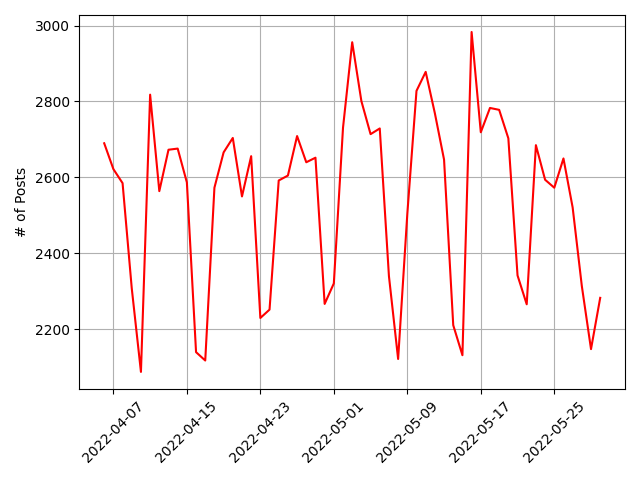
\includegraphics[width=0.75\textwidth]{Images/timeline.pdf}
    \caption{Number of daily posts across all subreddits}
    \label{fig:line-1}
\end{figure}

\par After storing data, an analysis tool runs to determine if a post is about crime. To do this, a regular expression checks if a post's title or a post's link's URL contains a crime-related keyword. These keywords were derived from actions that constitute violent crime and their synonyms, as well as generic crime-related words. In total, 46 keywords and their derivatives are used. If the regular expression returns a hit, a flag is raised in the database denoting that the post is about crime. Overall, 6,792 of the collected posts are estimated to discuss crime.

\par Due to the nature of text analysis, a number of false positives might be considered, while some false negatives go undetected. False negatives can be hard to detect, as they include dog-whistles, local-dependent terms, and ambiguous references (REF). Certain posters may choose to keep their posts ambiguous so as to keep their intentions visible to only a small group (REF).

\par To determine the rate of false positives, we analyze a sample of scraped posts. We look for phrases such as ``I shot a picture'' that do not relate to crime, but contain a crime-related keyword. Of a sample of 400 posts, we find that 36 posts do not relate to crime, for an accuracy rate of 91\%. Similar analysis done on the social media site reached a rate of 66\% \cite{curiel}.

\subsection{Contextual Data}
\par A variety of data were utilized to highlight trends in the Reddit posts. One variable that subreddits are compared to is population size of the MSA. These values range from a minimum of 58,639 (Carson City, NV) and a maximum of 20,140,470 (New York-Newark-Jersey City, NY-NJ-PA). MSAs are categorized into four bins based on their size: large, medium, small, and very small. The population cutoffs are 1,000,000, 500,000, and 200,000. The large population contains 56 members, the medium bin contains 54 members, the small bin contains 113 members, and the very small bin contains 161 members.

\par Another variable that provides context is the political climate of an MSA. For this, we consider the results of the 2020 election (REF) in terms of the percent of the MSA voting Democrat. These values range from a minimum of 20.2\% (Morristown, TN) to a maximum of 80.9\% (Santa Cruz-Watsonville, CA). The MSAs are categorized into five bins based on their voting results: Very Conservative, Conservative, Moderate, Liberal, and Very Liberal. The percentage cutoffs for the bins are 37.5\%, 47.5\%, 52.5\%, and 62.5\%. The Very Conservative bin contains 112 members, the Conservative bin contains 103 members, the Moderate bin contains 57 members, the Liberal bin contains 73 members, and the Very Liberal bin contains 39 members.

\par A third variable that is considered is the documented violent crime rate of each MSA. This data is derived from the FBI's Uniform Crime Reporting statistics (REF) \footnote{Data from the FBI mostly comes from the year that is most recent, 2019. However, not all municipalities report information, so there are slight estimations in the data (REF).}. These values range from a minimum of 44.3/100,000 (Bangor, ME) to a maximum of 1,397.2/100,000 (Birmingham-Hoover, AL). Documented crime data is also normalized using min-max normalization so that it can be compared to a similarly normalized crime discussion value from the Reddit data.

\section{Methods}
\par We use one main scraper to gather post data from Reddit. This scraper utilizes multiple different tools to gather disparate pieces of data and place them into two datastores. This scraper prioritizes resilience to ensure that all posts are accounted for. Additionally, the scraper checks for new posts once every hour so that posts can be fetched before a user deletes them or a moderator deletes them. These communities are generally slow moving, with an average of 111 posts an hour between all 384 subreddits.

\par To gather the data, the scraper first sends requests to the Reddit REST API \cite{reddit}. We use the \texttt{new} endpoint for each subreddit to check the most recent posts. The post last written to the database for each subreddit is cached in a database table so that we can take advantage of the \texttt{after} parameter of the API. This parameter allows us to take posts that have been created since a given post ID. This parameter is especially useful on slower subreddits; without it, we would be performing requests on posts that might be months old. If the cached value does not exist or is not valid, then the most recent hundred posts are gathered. This is the maximum allowable value by the Reddit API.

\par After performing error checking to ensure all of our requests went through, each record is sent to two databases. The first is a CockroachDB database that acts as a system of record. Raw posts are stored here in a simple format: \texttt{id}, \texttt{timestamp}, and \texttt{data}, which is the data retrieved from the Reddit API in JSON format. After writing to CockroachDB, the scraper then writes the JSON data from Reddit to ElasticSearch. ElasticSearch provides quick and efficient text analysis that allows for the extraction of certain keywords in post titles and URLs.

\par The scraper and databases run in Docker containers. Containerization allows the tool, as well as the databases, to run in a clean, isolated environment without worrying about being choked out by other processes. Additionally, the tool-container is scheduled by Kubernetes to allow for a higher degree of availability and resilience. If something unexpected occurs and the tool goes down, it will simply be restarted by Kubernetes.

\section{Results}

\subsection{Subreddit Activity}

\par In total, the Reddit scraper gathered 161,166 posts between 384 subreddits. Posts were collected between April 5th, 2022 to May 31, 2022. Table \ref{table:table-1} details the ten most active subreddits of those monitored. Similarly, Table \ref{table:table-2} lists the ten most active subreddits when normalized by population.

\begin{table}[h!]
    \centering
    \small
    \caption{Most active Metropolitan Areas}
    %\begin{tabu} to 1.0\textwidth {| *{3}{c|} }
    \begin{tabular}{| c | c | c |}
    \hline
    Metropolitan Statistical Area & Number of Posts & Population\\ \hline
    Austin-Round Rock-Georgetown, TX & 4,084 & 2,283,371 \\ \hline
    San Diego-Chula Vista-Carlsbad, CA & 3,265 & 3,298,634 \\ \hline
    Boston-Cambridge-Newton, MA-NH & 3,120 & 4,941,632 \\ \hline
    Denver-Aurora-Lakewood, CO & 2,785 & 2,963,821 \\ \hline
    Chicago-Naperville-Elgin, IL-IN-WI & 2,673 & 9,618,502 \\ \hline
    Sacramento-Roseville-Folsom, CA & 2,668 & 2,397,382 \\ \hline
    Philadelphia-Camden-Wilmington, PA-NJ-DE-MD & 2,541 & 6,245,051 \\ \hline
    Columbus, OH & 2,533 & 2,138,926 \\ \hline
    Portland-Vancouver-Hillsboro, OR-WA & 2,526 & 2,512,859 \\ \hline
    San Francisco-Oakland-Berkeley, CA & 2,476 & 4,749,008 \\ \hline
	\end{tabular}
	\label{table:table-1}
\end{table}

\par The most active MSAs by total number of posts share some common, predictable traits. One shared characteristic is that all of the Metropolitan Areas listed have populations above 1,000,000. While expected, some of the most notable MSAs were not included, such as New York-Newark-Jersey City, NJ-NJ-PA and Los Angeles-Long Beach-Anaheim, CA, which have populations of 20,140,470 and 13,200,998, respectfully. One possible explanation for these exclusions is the fact that there is no uniform, consistent moderation policy among subreddits (REF). For example, some subreddits automatically filter out all posts and manually approve them, or they disallow certain types of posts (REF - nyc n chicago rules). Subreddits with more laissez-faire moderation policies will have more posts simply because they are not removing a mass of posts that could be considered redundant or irrelevant.

\begin{table}[h!]
    \centering
    \small
    \caption{Most active Metropolitan Areas per population}
    %\begin{tabu} to 1.0\textwidth {| *{3}{c|} }
    \begin{tabular}{| c | c | c |}
    \hline
    Metropolitan Statistical Area & Number of Posts & Population\\ \hline
    Bellingham, WA & 1,381 & 226,847 \\ \hline
    Bloomington, IN & 799 & 161,039 \\ \hline
    Missoula, MT & 449 & 117,922 \\ \hline
    Bend, OR & 660 & 198,253 \\ \hline
    Burlington-South Burlington, VT & 546 & 171,415 \\ \hline
    Corvallis, OR & 298 & 95,184 \\ \hline
    Eugene-Springfield, OR & 1,183 & 382,971 \\ \hline
    Charlottesville, VA & 638 & 221,524 \\ \hline
    Ithaca, NY & 299 & 105,740 \\ \hline
    Asheville, NC & 1,312 & 469,015 \\ \hline
	\end{tabular}
	\label{table:table-2}
\end{table}

\par The list of most active MSAs when normalizing by population also share some common traits. These MSAs are generally politically liberal (REF) and have large college age populations (REF). Essentially, these areas have large populations of people that fall under Reddit's main demographic (REF) and, as a result, have correspondingly active communities.

\subsection{Crime Discussion}

\par To first understand the relationship between certain socio-economic variables and the rate of crime discussion, we must first look at crime discussion percentages independently. Of the 161,166 posts gathered, 6,792 are determined to discuss crime by matching certain crime-related keywords to post titles and URLs. Table \ref{table:table-3} lists the Metropolitan Areas with the largest percentage of crime discussion from the total number of posts.

\begin{table}[h!]
    \centering
    \small
    \caption{Metropolitan Areas with most crime discussion}
    %\begin{tabu} to 1.0\textwidth {| *{3}{c|} }
    \begin{tabular}{| c | c | c |}
    \hline
    Metropolitan Statistical Area & \% Crime Posts & \# Crime Posts \\ \hline
    Seattle-Tacoma-Bellevue, WA & 18.2 & 344 \\ \hline
    Anniston-Oxford, AL & 15.7 & 8 \\ \hline
    Lewiston-Auburn, ME & 15.4 & 14 \\ \hline
    Bay City, MI & 14.0 & 7 \\ \hline
    Lewiston, ID-WA & 13.0 & 7 \\ \hline
    Pine Bluff, AR & 12.5 & 4 \\ \hline
    Los Angeles-Long Beach-Anaheim, CA & 12.0 & 257 \\ \hline
    Portland-Vancouver-Hillsboro, OR-WA & 11.4 & 287 \\ \hline
    Rocky Mount, NC & 11.3 & 7 \\ \hline
    Decatur, AL & 10.9 & 7 \\ \hline
    New York-Newark-Jersey City, NY-NJ-PA & 10.7 & 196 \\ \hline
    Flint, MI & 9.7 & 10 \\ \hline
    Morristown, TN & 9.3 & 4 \\ \hline
    Sumter, SC & 9.3 & 5 \\ \hline
    Vallejo, CA & 8.8 & 9 \\ \hline
	\end{tabular}
	\label{table:table-3}
\end{table}

\par Furthermore, Figure \ref{fig:map-1} displays a map of all Metropolitan Areas by the percentage of crime posts submitted to their respective subreddits. The darker the shade of green, the more posts discuss crime. The average crime discussion percentage lays at 3.5\%.

\begin{figure}[ht]
    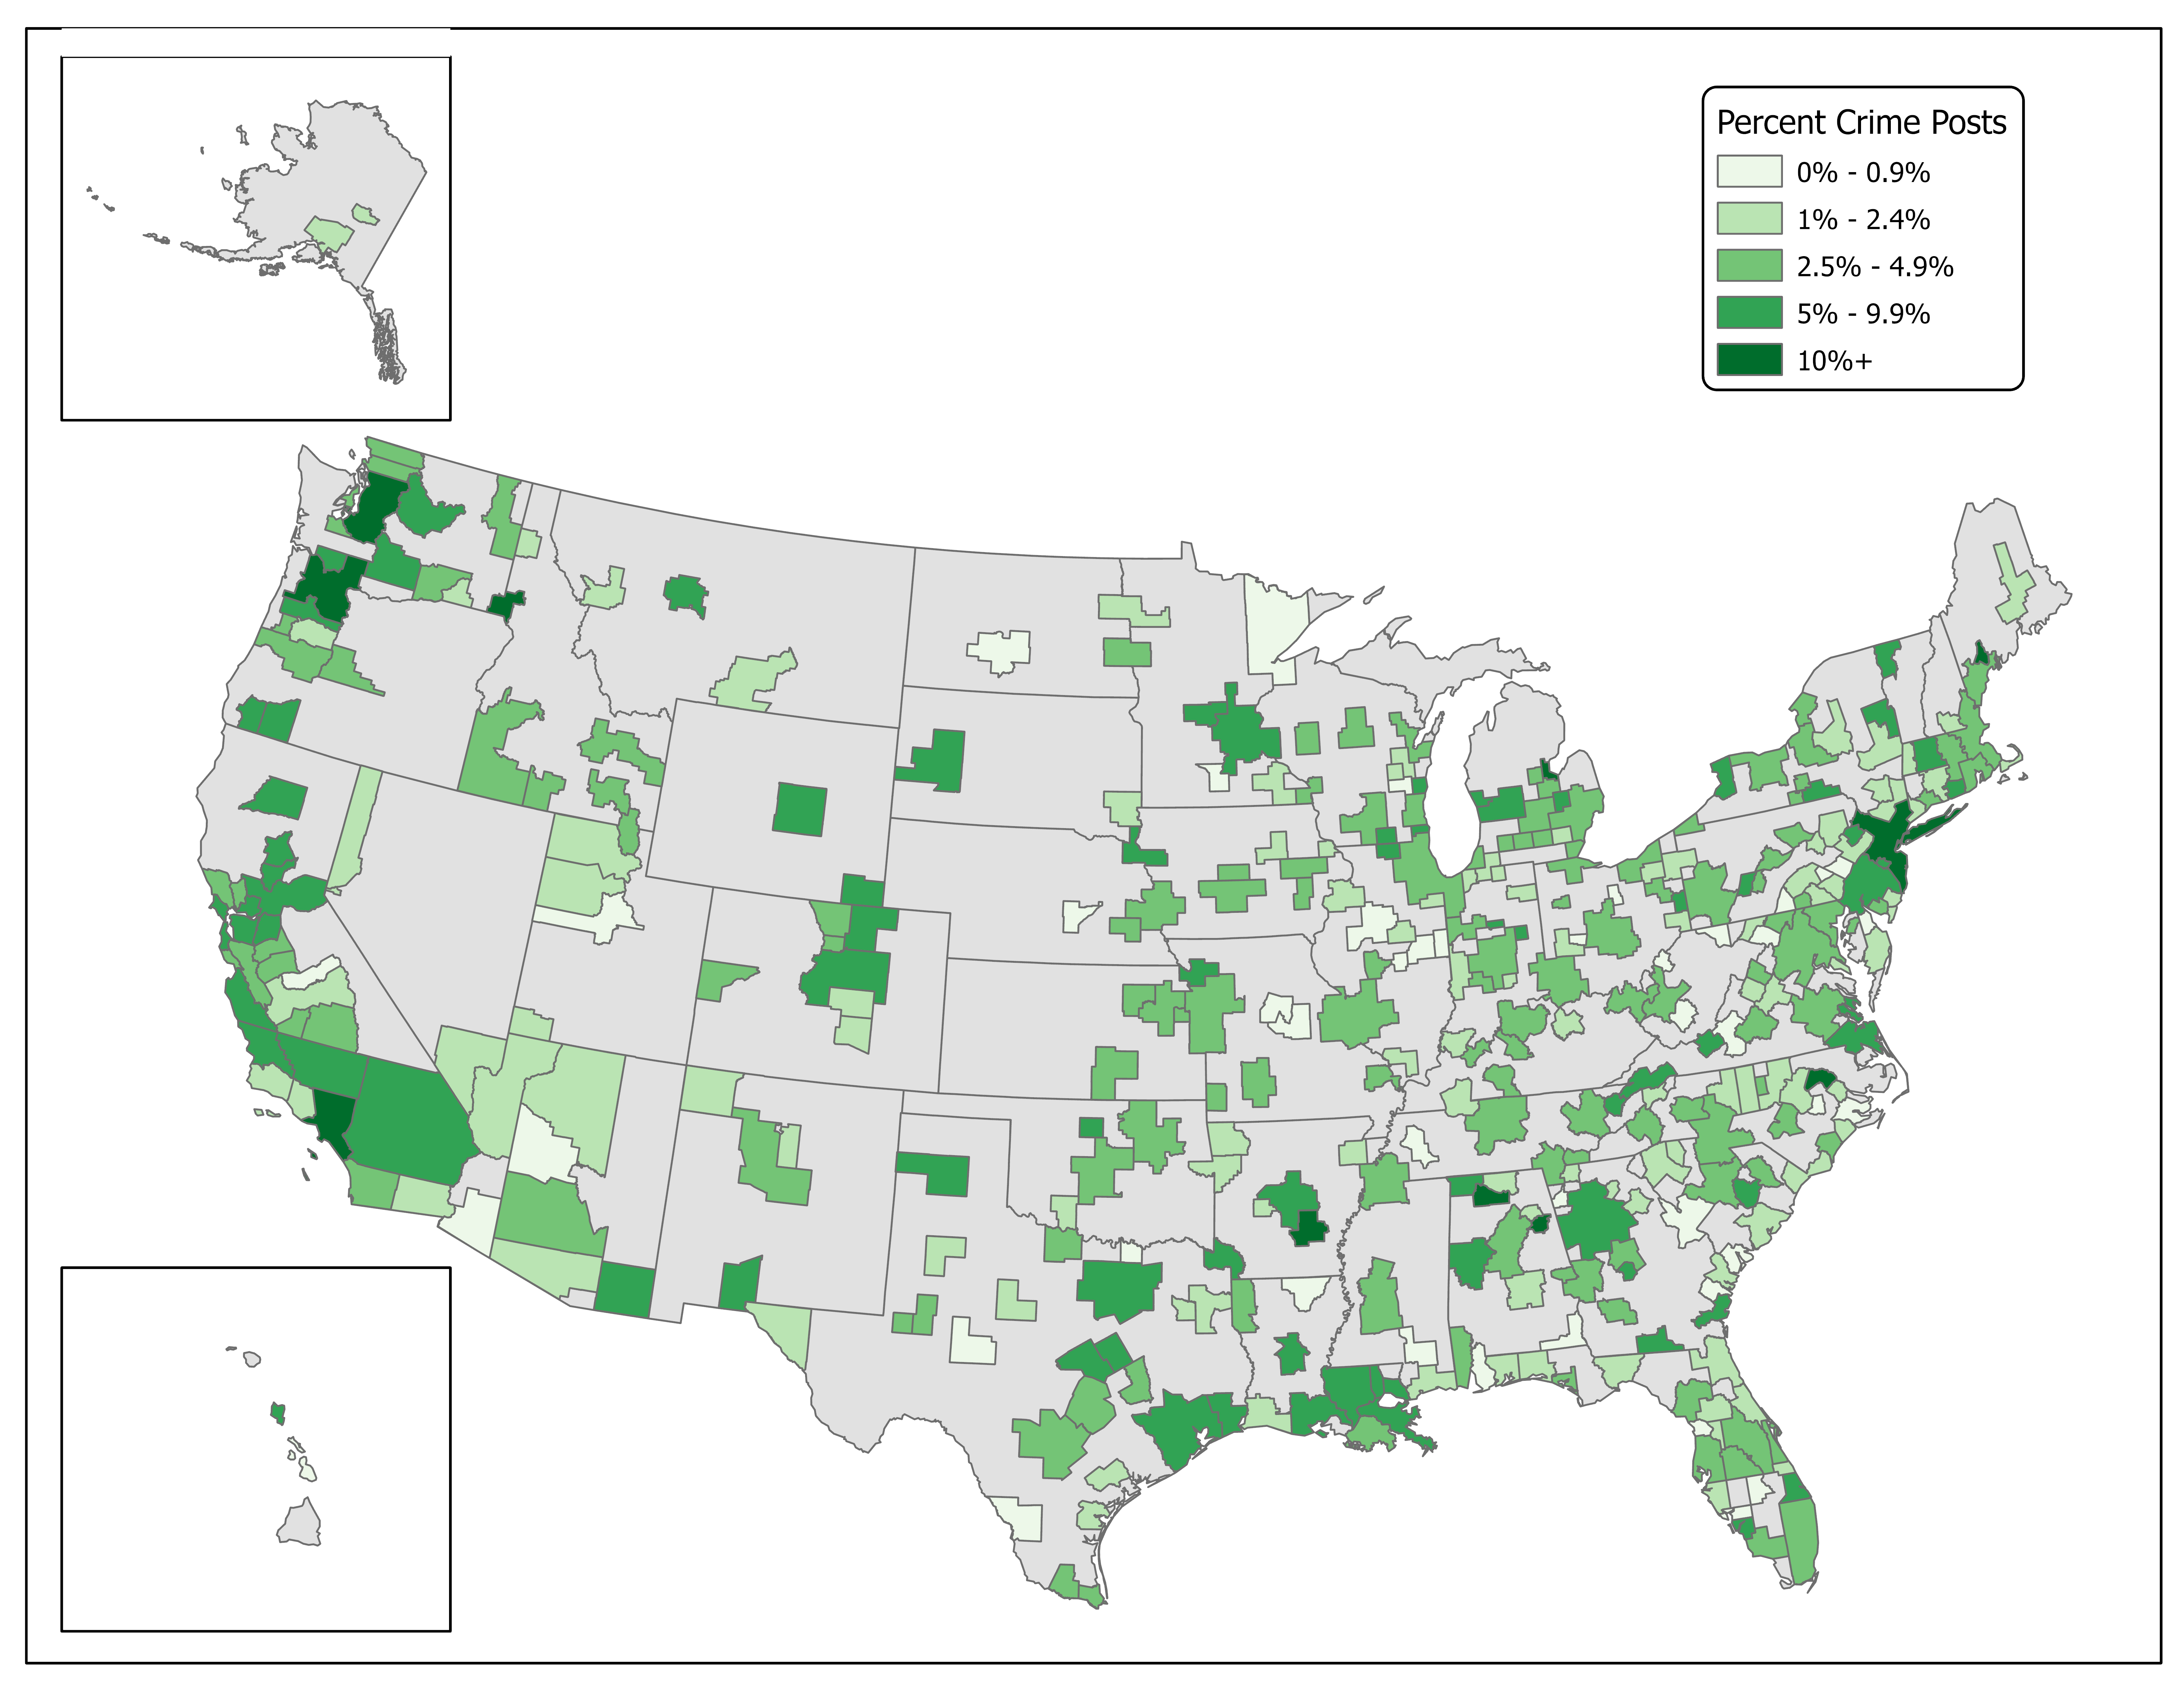
\includegraphics[width=\textwidth]{Images/PCrime.png}
    \caption{Map of crime discussion by MSA}
    \label{fig:map-1}
\end{figure}

\section{Contextual Analysis}

\subsection{Population Demographics}

\par The 384 MSAs of the United States vary greatly in terms of their actual population sizes. Once the Urban Area that makes the core of the Statistical Area reaches a population of at least 50,000, a Metropolitan Area forms in the county (or counties) that the Urban Area lies in. As a result of this definition, we break down MSAs into the four categories based on size discussed previously: very small, small, medium, and large. We use these categorizations to help explain trends in data relating to MSA population sizes.

\par To identify any potential trends in the population data, we take the mean crime discussion value of each bucket category. Figure \ref{fig:graph-1} displays the average min-max normalization score for the percentage of crime discussion based on population size. Here, the very small population bucket contains 161 members with an average normalized score of 0.196, the small bucket contains 113 members with an average score of 0.173, the medium bucket contains 54 members with an average score of 0.166, and the large bucket contains 56 members with an average score of 0.260.

\begin{figure}[ht]
    \centering
    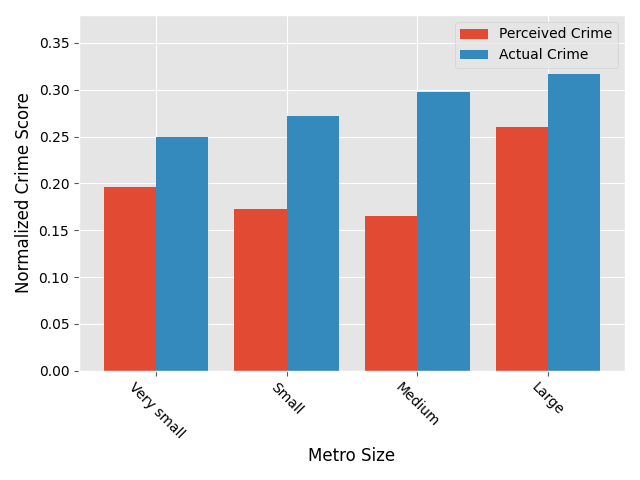
\includegraphics[width=0.75\textwidth]{Images/bar-population.pdf}
    \caption{Comparison of discussed crime and documented crime by population}
    \label{fig:graph-1}
\end{figure}

\par From Figure \ref{fig:graph-1}, we can see that as population increases, documented crime rates gradually increase. This trend is semi-reflected in the crime discussion data. Crime discussion scores are roughly equivalent for the very small, small, and medium buckets. However, the large population bucket has a significantly higher crime discussion score than that of the other buckets. The large population bucket has a 6\% greater score than the medium population bucket when comparing documented crime data, but the large population bucket has a 56\% greater score than the medium population bucket when comparing crime discussion data.

\par Figure \ref{fig:cdf-1} shows a cumulative distribution function of the data by population bucket. Here, we can see that the smallest value of the class of large populations is the greatest among the four classes, while its largest value is greater than all of the other classes' largest values. This relationship remains true throughout most of the distribution, resulting in the large MSAs having the highest mean crime discussion score. When looking at the very small MSAs, we can see that some Metropolitan Areas in its category have high average crime discussion. However, a significant amount of very small MSAs have no crime discussion at all. From the CDF we can see that almost 20\% of very small MSA subreddits have not discussed crime at all. The next highest zero crime discussion class is small, with about 8\% of communities not discussing crime.

\begin{figure}[ht]
    \centering
    \includegraphics[width=0.75\textwidth]{Images/cdf.pdf}
    \caption{Crime discussion by MSA population class}
    \label{fig:cdf-1}
\end{figure}

\par When looking back at the map of crime discussion in Figure \ref{fig:map-1}, we can see that the Metropolitan Areas with the most crime discussion are not bound by population size. MSAs both small and large are represented. However, this trend is not reflected among Metropolitan Areas with the least amount of crime discussion. These areas are almost exclusively in the very small and small population buckets, with no large population MSAs being represented. Having at least some degree of crime discussion in all MSAs and significant representation in the highest scoring MSAs leads to large population Metropolitan Areas scoring the greatest average crime discussion among all population classes.

\subsection{Political Atmosphere}

\par Similarly to population data, political affiliation is one possible variable that can sway crime discussion. To measure this, we look at the results of the 2020 presidential election. We consider the number of votes that the Democratic and Republican parties received as stand-ins for liberal and conservative political views, respectfully. Political affiliation of the 384 MSAs is broken down into the five categories discussed earlier: very conservative, conservative, moderate, liberal, and very liberal. Figure \ref{fig:map-2} shows a map of the political affiliation of all Metropolitan Areas in the United States.

\begin{figure}[ht]
    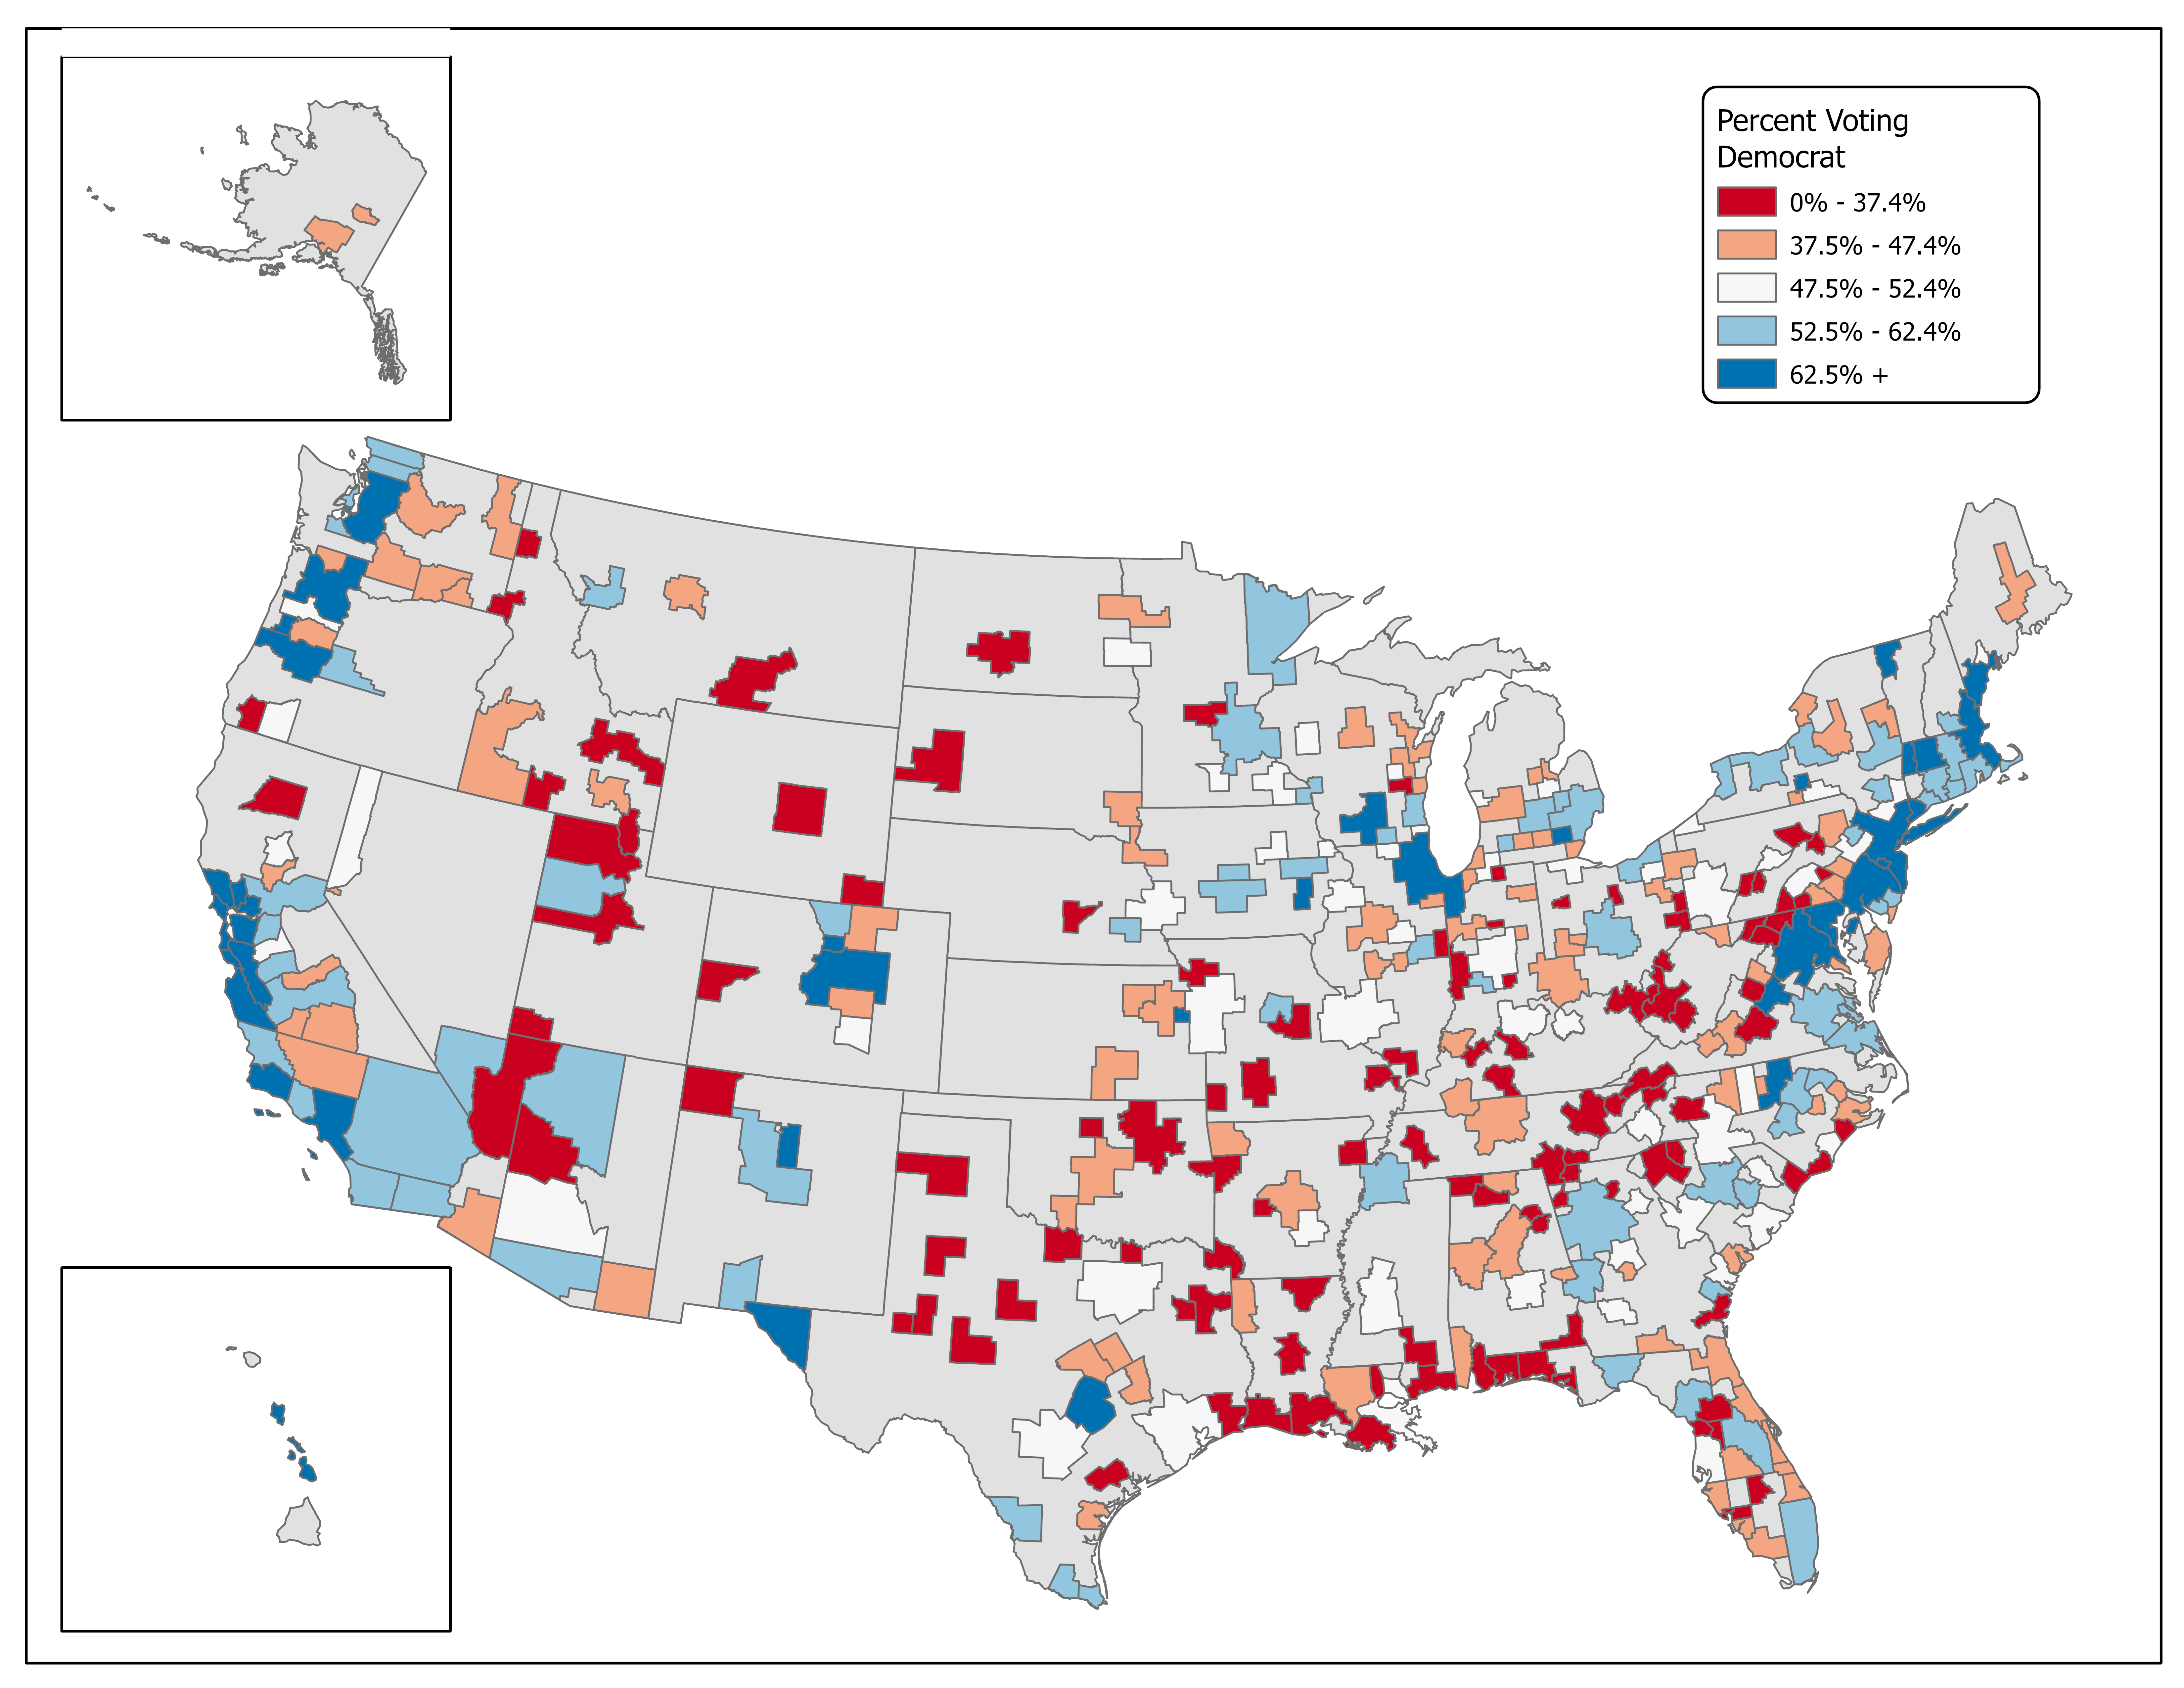
\includegraphics[width=\textwidth]{Images/pol.png}
    \caption{Map of 2020 presidential election results by MSA}
    \label{fig:map-2}
\end{figure}

\par In identifying trends based on politics, we follow a familiar method; we take the mean normalized crime discussion value and mean normalized documented crime rate of each political class. Figure \ref{fig:graph-2} displays the average min-max normalization score for crime discussion and reported crime for each political class. Here, the very conservative bucket contains 112 members with a mean score of 0.170, the conservative bucket contains 103 members with a mean score of 0.179, the moderate bucket contains 57 members with a mean score of 0.207, the liberal bucket contains 73 members with a mean score of 0.201, and the very liberal bucket contains 39 members with a mean score of 0.274.

\begin{figure}[ht]
    \centering
    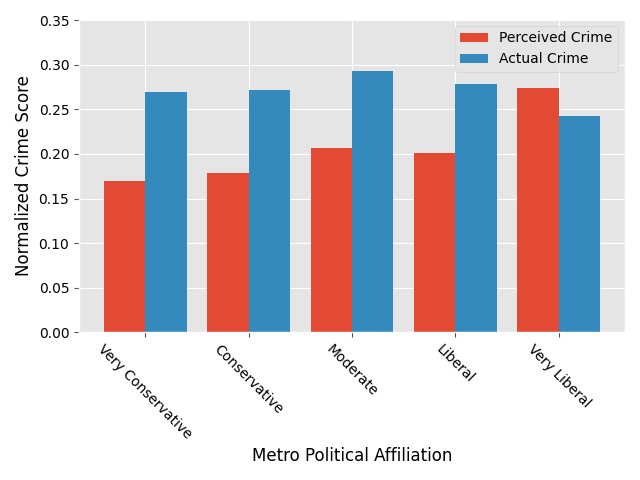
\includegraphics[width=0.75\textwidth]{Images/bar-politics.pdf}
    \caption{Comparison of discussed crime and documented crime by political class}
    \label{fig:graph-2}
\end{figure}

\par When looking at Figure \ref{fig:graph-2}, we can see that among crime discussion rates, more liberal cities have the highest average scores. As the share of democratic voters increase, the average crime discussion score increases, with moderate MSAs scoring slightly higher than liberal MSAs. The very liberal class has a 32\% higher crime discussion score than the next largest score. Additionally, the two conservative political classes have the lowest mean crime discussion scores. However, these trends are not reflected in the documented crime rate scores. Figure \ref{fig:graph-2} shows that very liberal MSAs have a lower mean documented crime rate than more conservative areas, as well as the lowest mean score overall. Very liberal areas are also the only class in which the crime discussion score is higher than the reported crime rate score despite its low average documented crime.

\begin{figure}[ht]
    \centering
    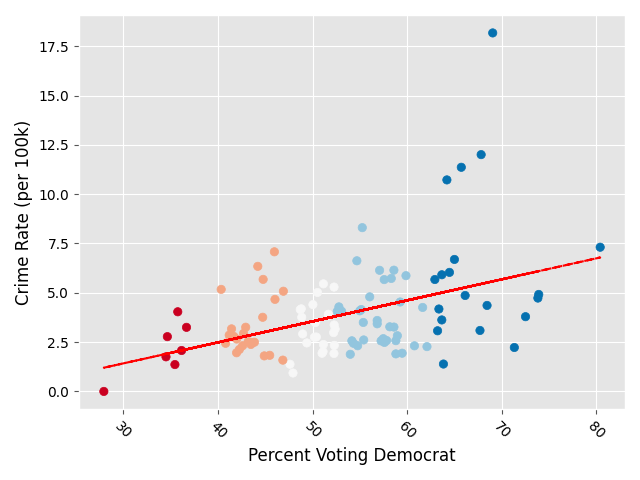
\includegraphics[width=0.75\textwidth]{Images/scatter-politics-mid-large.pdf}
    \caption{Crime discussion by percent voting Democrat}
    \label{fig:scatter-1}
\end{figure}

\par Figures \ref{fig:scatter-1} and \ref{fig:scatter-2} show two scatterplots: one which shows the percent crime discussion in relation to politics among medium and large sized MSAs and the other which shows the documented crime rate among the same sample group in relation to politics. The shades of the dots represent their political class. From the trendline in the data, we can see that as areas become more liberal, their crime discussion percentages increase fairly rapidly. The most conservative member of the plot, Provo-Orem, UT, did not include a single post discussing crime, while more liberal areas such as Seattle, Los Angeles, Portland, and New York City had values over 10\%. In contrast, when looking at the documented violent crime rate among large and mid-size MSAs, more liberal areas generally have lower average crime rates. MSAs that lean conservative, such as Birmingham-Hoover, AL and Kansas City, MO-KS have among the highest crime rates, as well as more politically moderate cities, such as Memphis, TN-MS-AR.

\begin{figure}[ht]
    \centering
    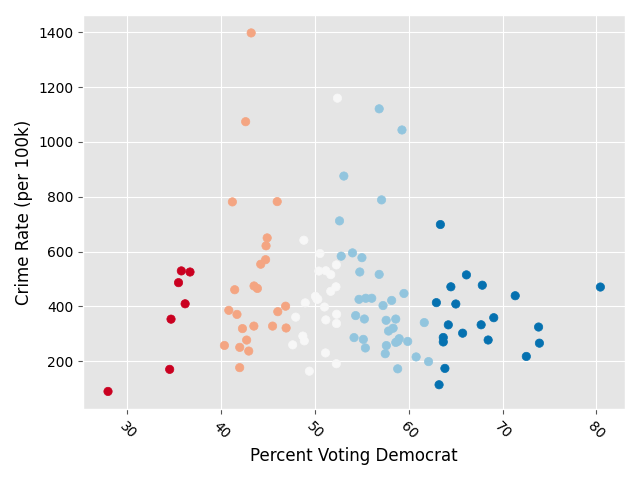
\includegraphics[width=0.75\textwidth]{Images/scatter-crime-mid-large.pdf}
    \caption{Crime discussion by documented crime rate}
    \label{fig:scatter-2}
\end{figure}

\par When considering the data, we can see a strong relationship between how liberal a Metropolitan Area votes to how high its average crime discussion lies. Despite having lower than average documented crime, very liberal Metropolitan Areas have the highest crime discussion rates.

\subsection{Reported Crime}

\par Another factor to consider alongside crime discussion is the reported crime rate of an MSA. Higher documented crime rates can lead to increased amounts of crime discussion, as crime may affect more members of the community. To measure MSA crime rates, we use the FBI's Uniform Crime Reporting Estimates (REF). The 384 Metropolitan Areas represent a differing level of crime rates, with a high of 1397.2 from Birmingham-Hoover, AL, a low of 44.3 from Bangor, ME, and an average of 380.9 among all MSAs. Table \ref{table:table-3} displays the MSAs with the ten highest documented crime rates. In this case, crime rates are defined as the amount of violent crime per 100,000 people. Additionally, the map in Figure \ref{fig:map-3} displays the crime rate for all Metropolitan Areas.

\begin{table}[h!]
    \centering
    \small
    \caption{Most active Metropolitan Areas per population}
    %\begin{tabu} to 1.0\textwidth {| *{3}{c|} }
    \begin{tabular}{| c | c | c |}
    \hline
    Metropolitan Statistical Area & Crime Rate & \% Crime Discussion\\ \hline
    Birmingham-Hoover, AL & 1,397.2 & 2.52 \\ \hline
    Farmington, NM & 1199.8 & 1.61 \\ \hline
    Anchorage, AK & 1194.6 & 2.36 \\ \hline
    Kansas City, MO-KS & 1159.4 & 3.16 \\ \hline
    Memphis, TN-MS-AR & 1120.5 & 3.43 \\ \hline
    Winston-Salem, NC & 1073.6 & 2.32 \\ \hline
    Albuquerque, NM & 1043.4 & 4.53 \\ \hline
    Danville, IL & 935.7 & 0.00 \\ \hline
    Pine Bluff, AR & 895.4 & 12.5 \\ \hline
    Odessa, TX & 881.8 & 4.30 \\ \hline
	\end{tabular}
	\label{table:table-4}
\end{table}

\par Table \ref{table:table-4} represents a diverse group of Metropolitan Areas in regards to population, politics, and crime discussion rates. Populations range from very small MSAs to large MSAs. Most of the MSAs lean conservative, but there are some liberal cities included, such as Albuquerque, NM. Additionally, a wide array of crime discussion percentages are noted, including Danville, IL at a low of 0\% and Pine Bluff, AR at a high of 12.5\%.

\begin{figure}[ht]
    \centering
    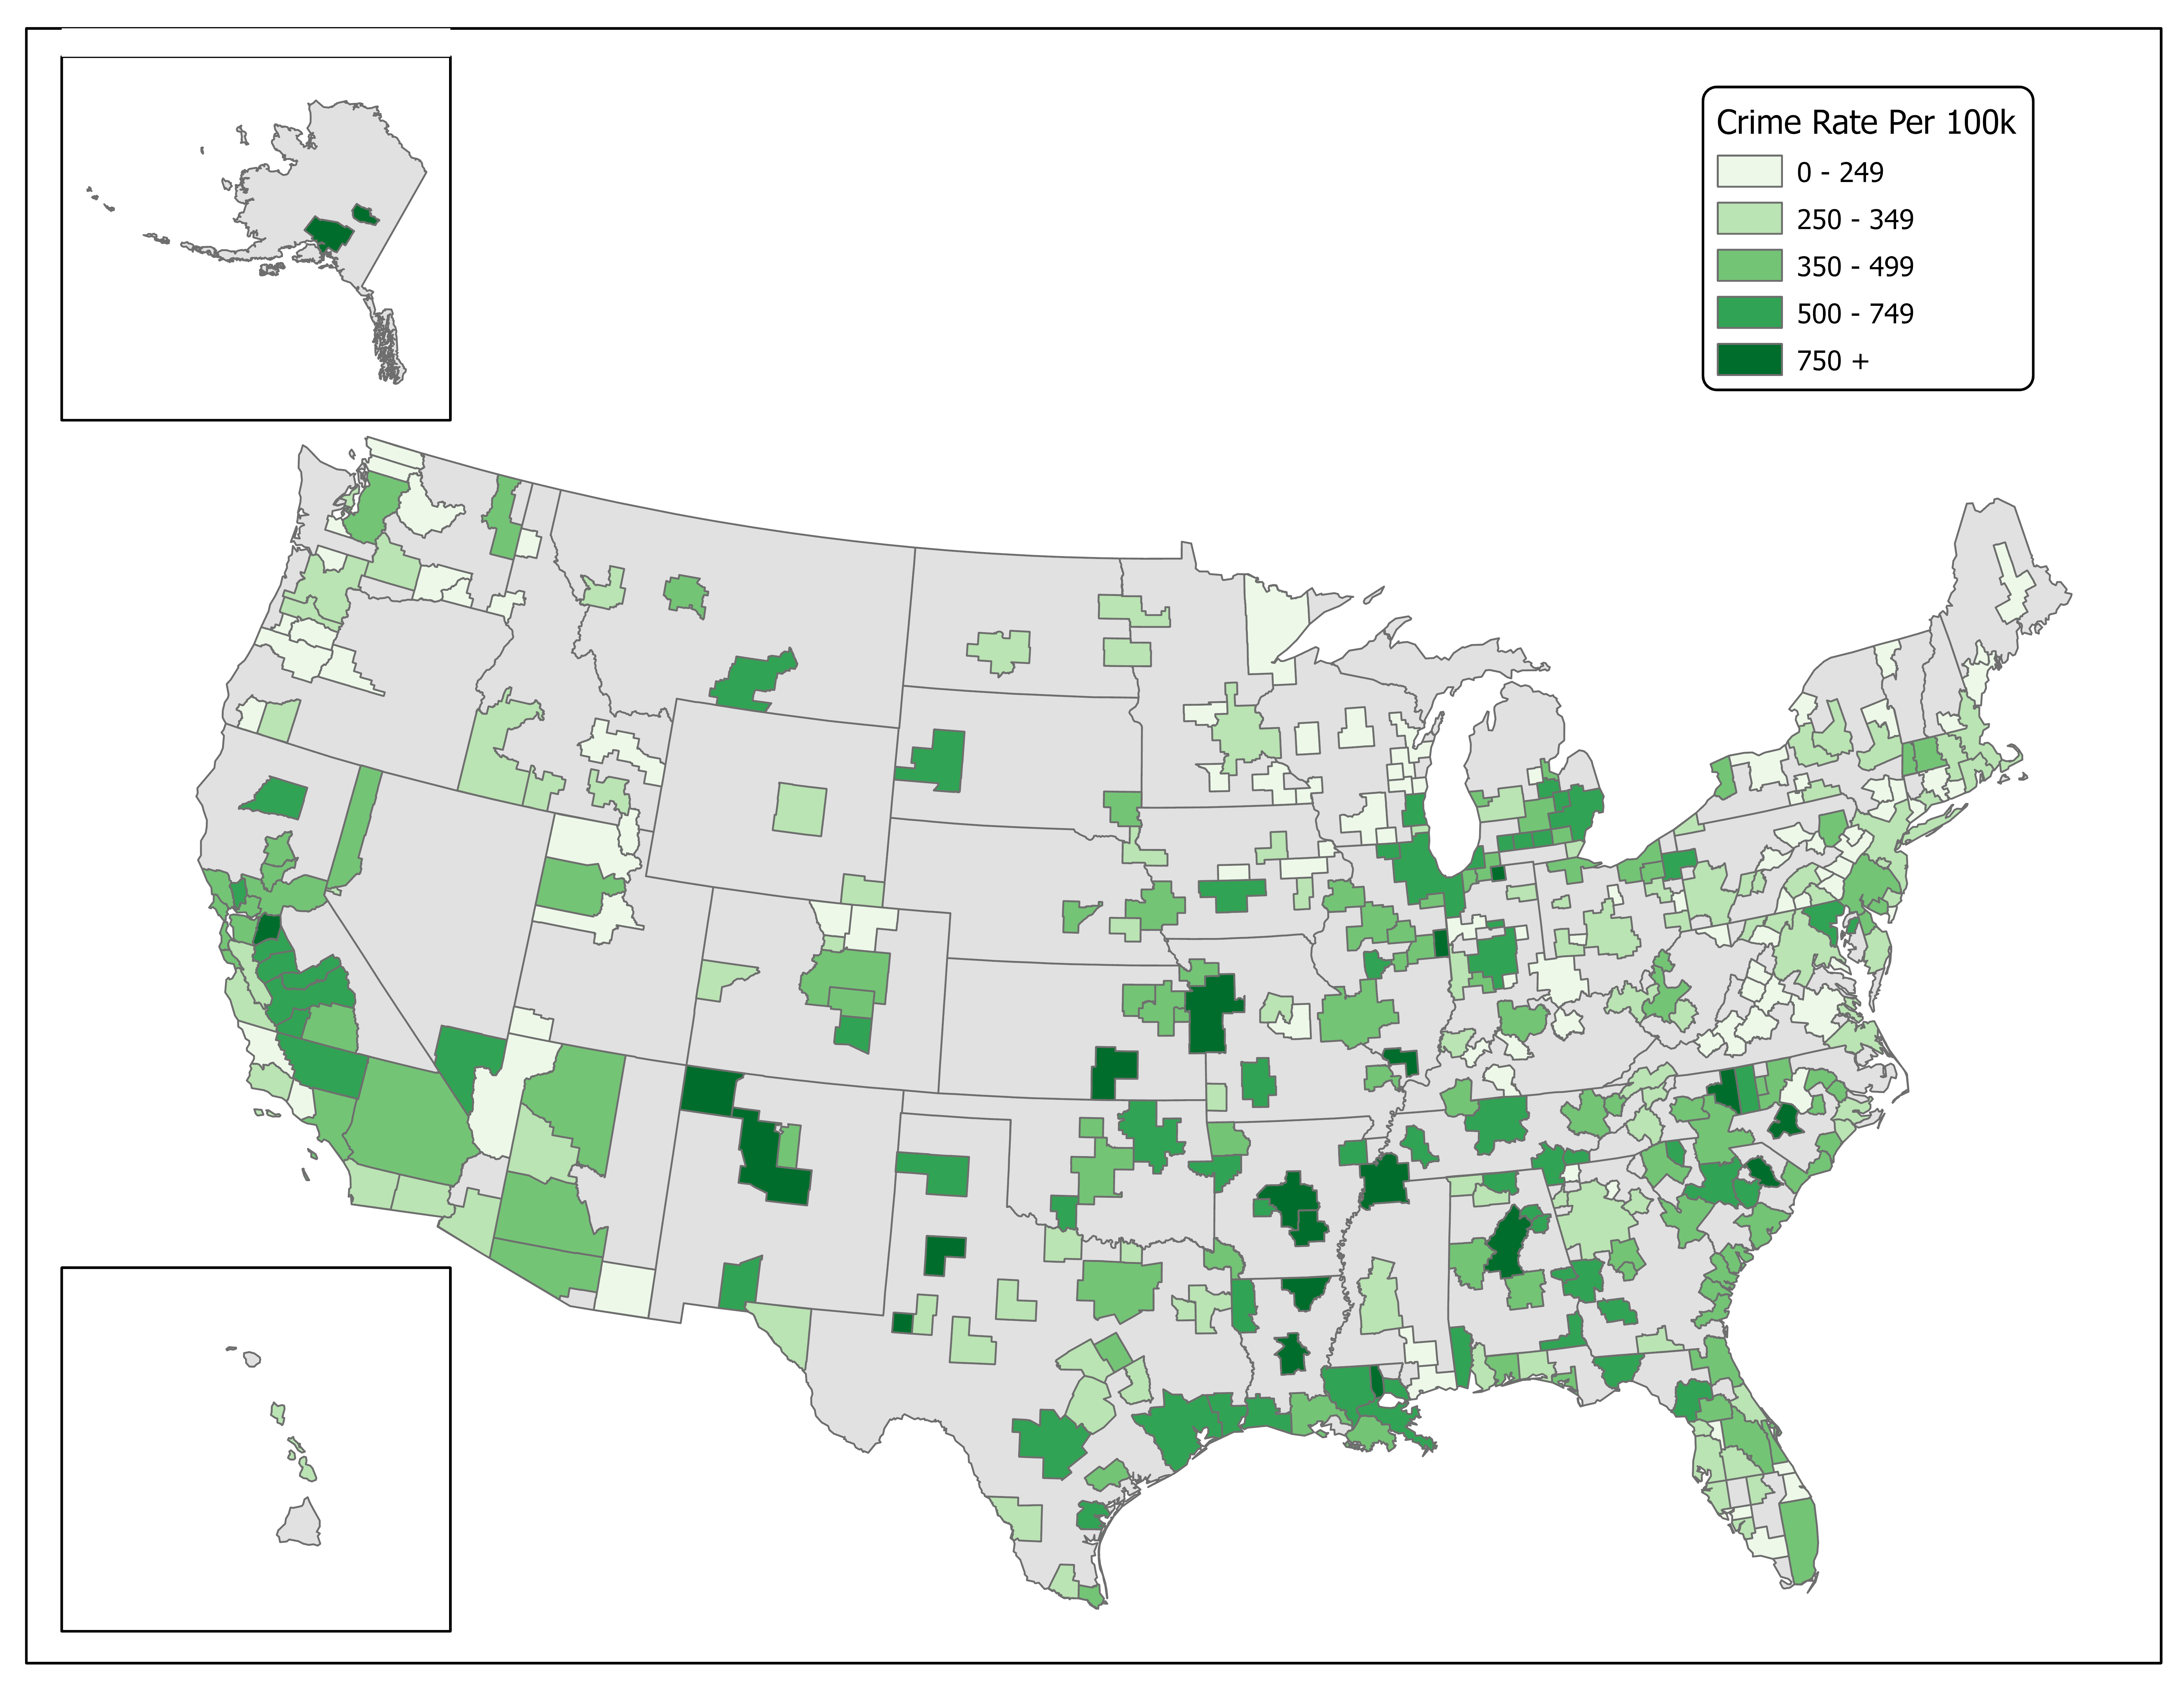
\includegraphics[width=\textwidth]{Images/Crime.png}
    \caption{Reported Crime Rate by MSA}
    \label{fig:map-3}
\end{figure}

\par From Tables \ref{table:table-3} and \ref{table:table-4}, as well as Figures \ref{fig:map-1} and \ref{fig:map-3}, we can see that MSAs with high reported crime rates do not necessarily have high amounts of crime discussion. This includes Metropolitan Areas such as Danville, IL and Farmington, NM. The same goes for MSAs with low crime rates and low amounts of crime discussion. New York-Newark-Jersey City, NY-NJ-PA and Seattle-Tacoma-Bellevue, WA have significantly higher normalized crime discussion rates than normalized documented crime rates.

\begin{figure}[ht]
    \centering
    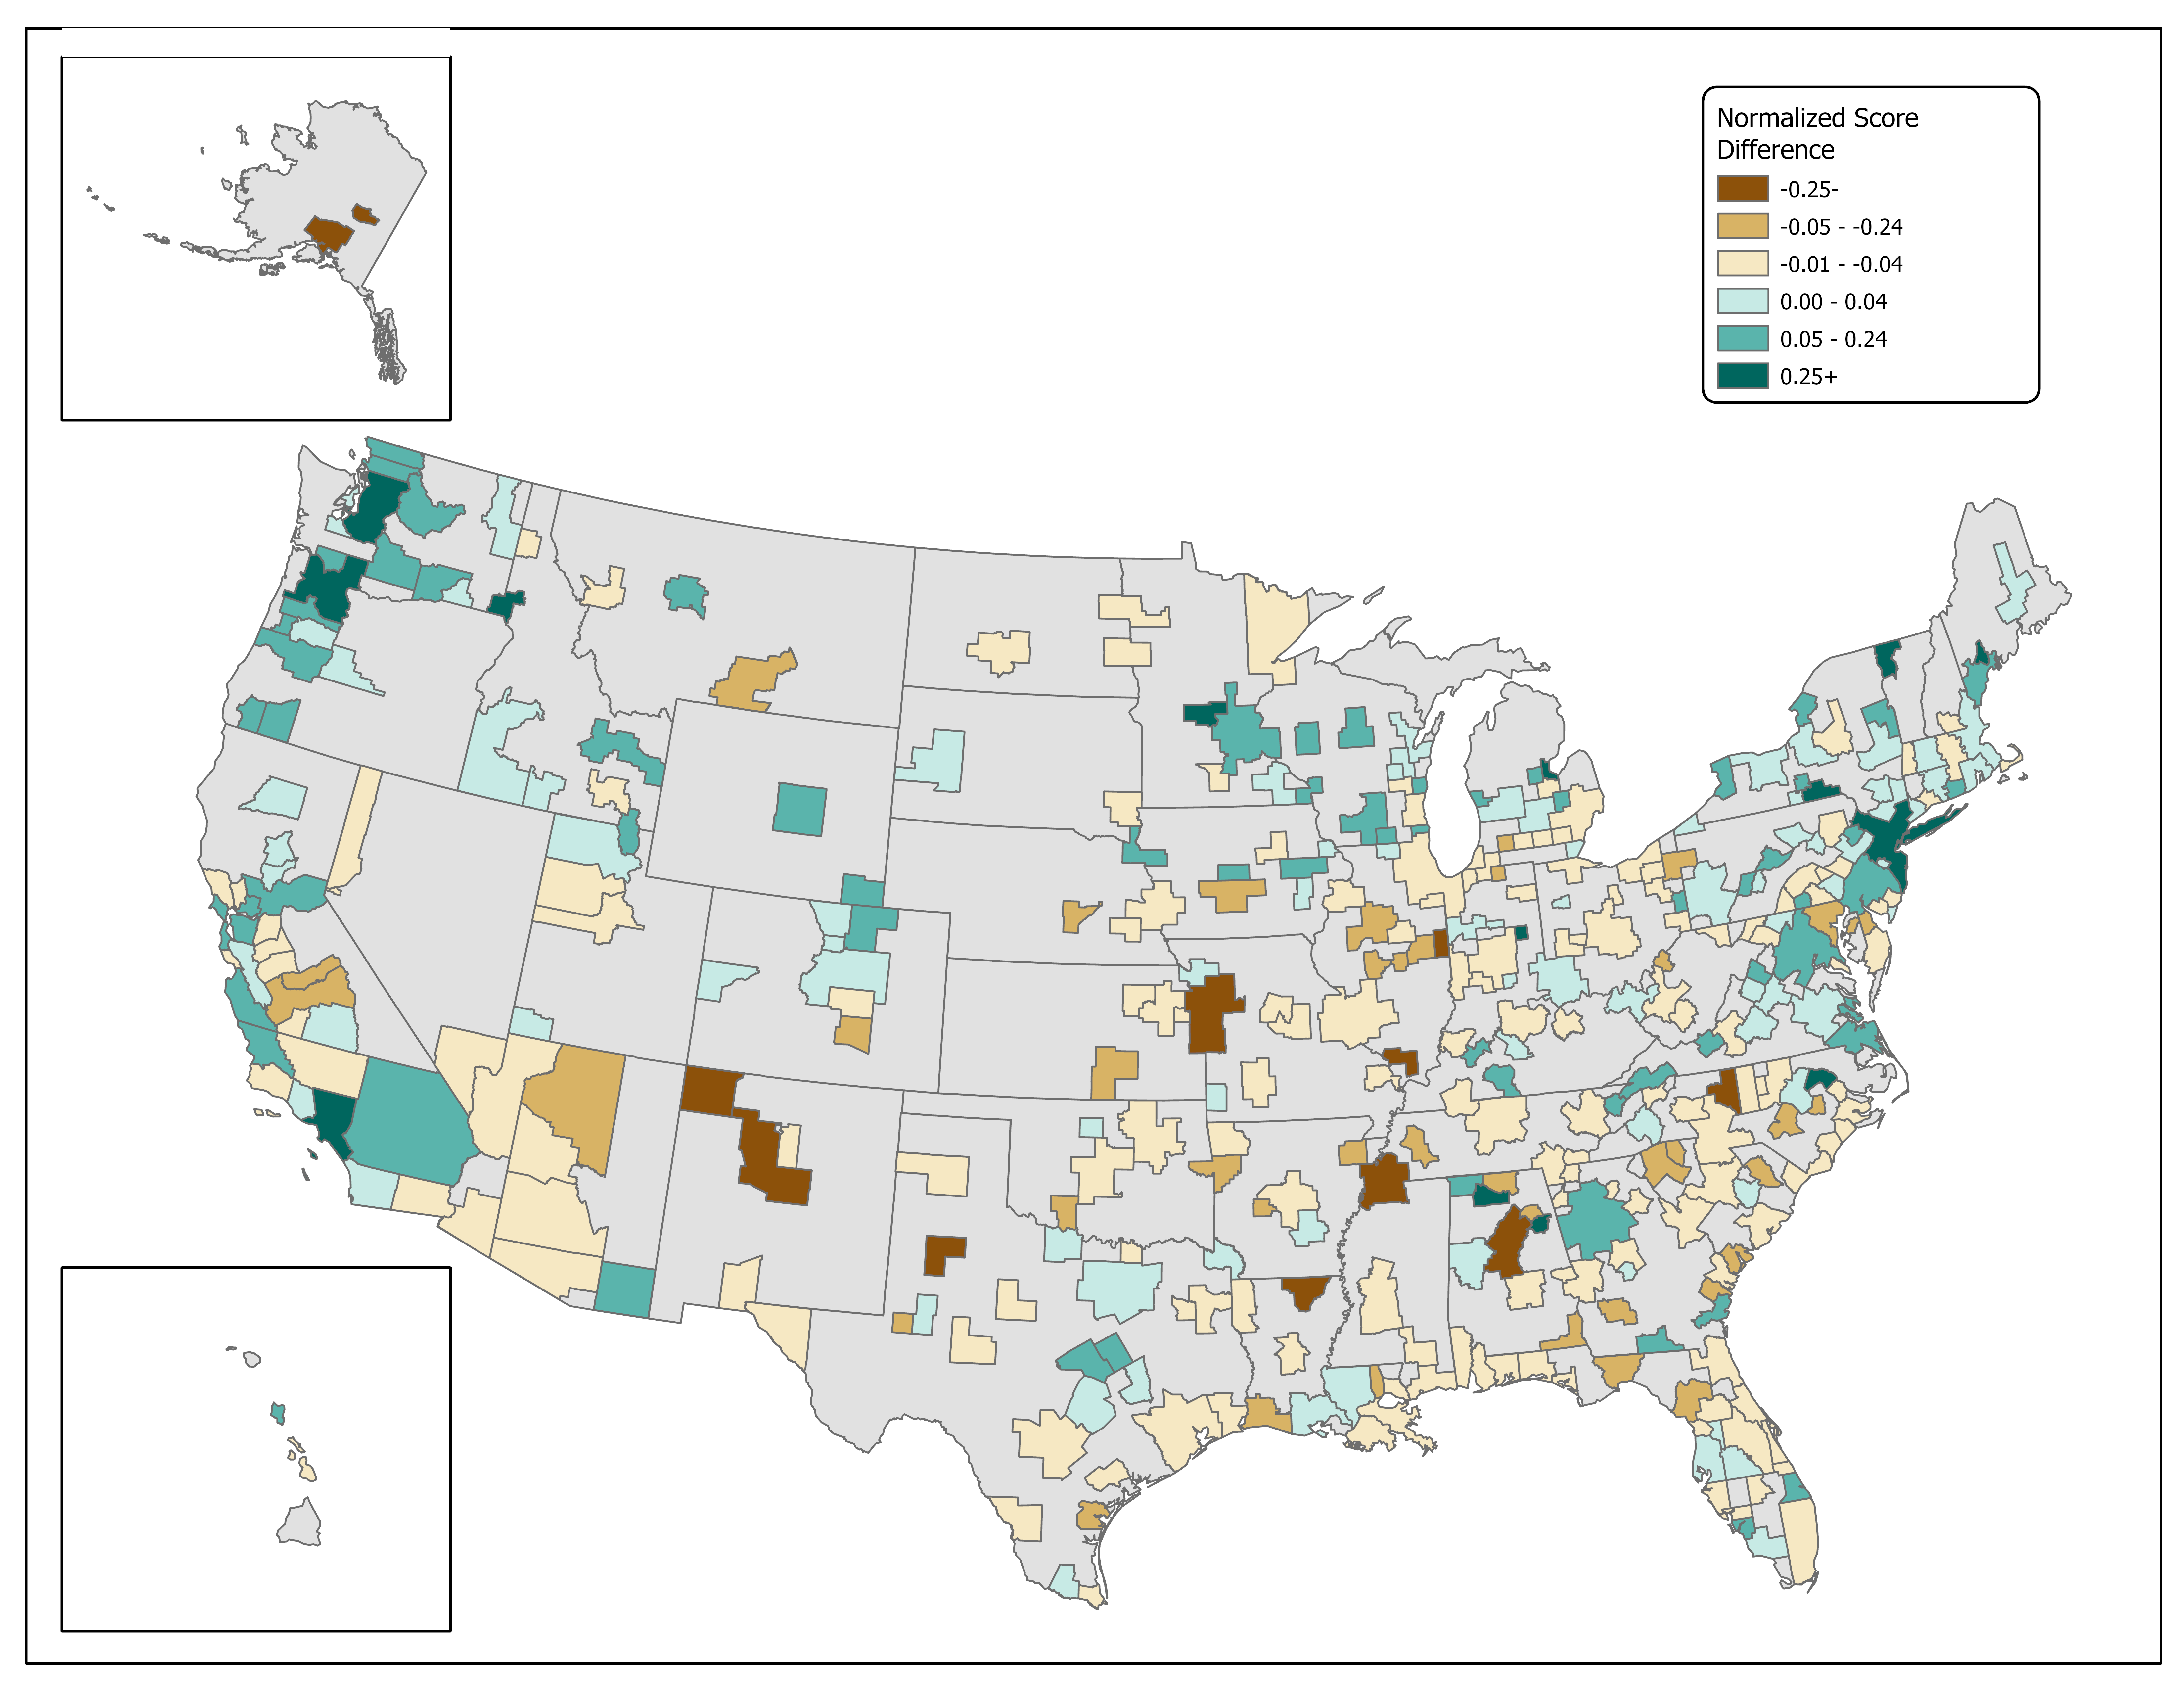
\includegraphics[width=\textwidth]{Images/diff.png}
    \caption{Reported Crime Rate by MSA}
    \label{fig:map-4}
\end{figure}

\par From the map in Figure \ref{fig:map-3}, we can see that many Metropolitan Areas with high documented crime rates lie in the South and Midwest (REF). However, many these MSAs have low amounts of crime discussion. To calculate the discrepancies between crime discussion and reported crime, we calculate the difference between the min-max normalized crime discussion score and the min-maxed documented crime score. Figure \ref{fig:map-4} maps this normalized difference score. Higher positive values indicate that the amount of crime discussion is higher than actual crime, while lower negative values indicate that actual crime is higher than crime discussion. MSAs in which the ratio of crime discussion and documented crime are roughly equal rest around a score of zero.

\par Table \ref{table:table-5} displays the 15 highest and lowest scoring MSAs for the crime discussion to crime rate ratio. A full listing can be found in Appendix (REF). Of the highest scoring MSAs, large and very small Metropolitan Areas are over-represented, while all population sizes are represented among the lowest scoring Metropolitan Areas. When considering political affiliation, very liberal cities represent 33\% of the highest scoring MSAs while only consisting of 10\% of the total number of Metropolitan Areas. For the lowest scoring MSAs, conservative and very conservative Metropolitan Areas represent 80\% of the lowest scoring members while only making up 56\% of the total number of members.

\begin{table}[h!]
    \centering
    \caption{MSAs by highest and lowest difference score}
    %\begin{tabu} to 1.0\textwidth {| *{3}{c|} }
    \begin{tabular}{| c | c | c | c |}
    \hline
    \multicolumn{2}{|c|}{Higher Score} & \multicolumn{2}{|c|}{Lower Score} \\ \hline
    Metropolitan Area & Score & Metropolitan Area & Score \\ \hline
    Seattle-Tacoma-Bellevue, WA & 0.743 & Birmingham-Hoover, AL & -0.861 \\ \hline
    Lewiston, ME & 0.723 & Farmington, NM & -0.770 \\ \hline
    Lewiston, ID-WA & 0.614 & Anchorage, AK & -0.725 \\ \hline
    Bay City, MI & 0.496 & Danville, IL & -0.670 \\ \hline
    Portland, OR-WA & 0.409 & Kansas City, MO-KS & -0.656 \\ \hline
    Decatur, AL & 0.381 & Winston-Salem, NC & -0.641 \\ \hline
    New York, NY-NJ-PA & 0.352 & Memphis, TN-MS-AR & -0.613 \\ \hline
    Anniston, AL & 0.344 & Monroe, LA & -0.582 \\ \hline
    Rocky Mount, NC & 0.323 & Carbondale, IL & -0.501 \\ \hline
    Los Angeles, CA & 0.319 & Albuquerque, NM & -0.497 \\ \hline
    St. Cloud, MN & 0.308 & Fairbanks, AK & -0.490 \\ \hline
    Burlington, VT & 0.290 & Lubbock, TX & -0.489 \\ \hline
    Binghamton, NY & 0.273 & Corpus Christi, TX & -0.448 \\ \hline
    Muncie, IN & 0.262 & Jackson, TN & -0.439 \\ \hline
    Sheboygan, WI & 0.238 & Dothan, AL & -0.431 \\ \hline
	\end{tabular}
	\label{table:table-5}
\end{table}

\par When considering the documented crime data, we can see that high documented crime rates do not necessarily lead to high crime discussion rates, and vice versa. Figure \ref{fig:map-4} and Table \ref{table:table-5} show that more liberal and larger MSAs in the Northeast and on the West Coast have higher rates of crime discussion than crime rates, while smaller, more conservative MSAs in the South and Midwest have higher crime rates than crime discussion. As a result of these differing scores, no relationship between crime discussion and reported crime rates emerges.

\section{Sentiment Analysis and Overlap}

\par From the data collected by our Reddit scraper, we have seen that crime discussion is widespread among the selected communities. However, while we have analyzed posts about crime, we have not yet analyzed the users that initiate this crime discussion. In doing so, we can potentially identify trends in the data that could highlight motivations behind crime posters or their submission patterns. We can also attempt to identify if crime posters are truly local by seeing if they overlap with other state and local subreddits. 

\par To analyze users' posting histories, we extract their submission and comment data. For this work, we use posters to \texttt{r/nyc}, the New York City subreddit as a sample. We have extracted all 1,197 unique posters from the 1,828 posts to \texttt{r/nyc}. 134 of these posters have posted about crime at least once, while 1,063 have not. Seven users have posted about crime five or more times. Additionally, of the 134 crime posters, five have had their account suspended since May 31st, 2022. This accounts for 3.7\% of the crime posters. Of the 1,063 non-crime posters, 27 have had their accounts suspended, or 2.5\%. After fetching the unique users, we gathered posts and comments from their user history. In total, 11,926 comments and posts were gathered from crime-posting users, while 87,658 comments and posts were gathered from non-crime-posting users.

\par One method of measuring user interaction patterns is through performing sentiment analysis on post and comment data. In this case, we measure the mean polarity score of users who post about crime and compare it to the mean polarity score of users who don't post about crime. A lower polarity means that the input data is more negative, while higher scores mean that the sentiment is more positive (REF). This can indicate the potential nature of a poster; if their polarity score is low, then they are a consistently negative voice in the community. Enough negative voices can detract from a community and introduce conflict and disarray.

\begin{table}[h!]
    \centering
    \small
    \caption{Sentiment polarity scores for \texttt{nyc} users}
    %\begin{tabu} to 1.0\textwidth {| *{3}{c|} }
    \begin{tabular}{| c | c | c |}
    \hline
     & Crime posters & Non-crime posters \\ \hline
    Within \texttt{r/nyc} &  -0.07 & 0.09 \\ \hline
    Outside of \texttt{r/nyc} & -0.07 & 0.10 \\ \hline
	\end{tabular}
	\label{table:table-6}
\end{table}

\par Table \ref{table:table-6} displays the results of the sentiment analysis on users that submitted a post to the New York City subreddit. Comments and posts were divided between those within \texttt{r/nyc} and those outside of the community. The sentiment of crime-posters was nearly identical within and outside of the community. These poster were more on the negative side, with neutrality laying at zero. Non-crime posting users were generally more positive, scoring 0.09 within the community and 0.10 outside of the community.

\par Another method of analyzing user interaction patterns is through identifying other communities that \texttt{r/nyc} members post in. This can potentially identify important posting trends. Examples include location identity and political affiliation. To measure this, we use the Jaccard Index. The Jaccard index can be defined as:

(REF)

\par Table \ref{table:table-7} displays the subreddits with the highest overlap for both crime and non-crime posters. Crime posters and non-crime posters alike share some common, New York City-related subreddits, such as \texttt{NYCBike}. However, crime posters have high overlap between two subreddits specifically meant to discuss crime in New York City: \texttt{CrimeInNYC} and \texttt{NYStateOfMind}.

\begin{table}[h!]
    \centering
    \small
    \caption{Subreddits with highest overlap by poster type}
    %\begin{tabu} to 1.0\textwidth {| *{3}{c|} }
    \begin{tabular}{| c | c | c | c |}
    \hline
    \multicolumn{2}{|c|}{Crime poster} & \multicolumn{2}{|c|}{Non-crime poster} \\ \hline
    Subreddit & Score & Subreddit & Score\\ \hline
    \texttt{CrimeInNYC} & 0.83 & \texttt{nycrail} & 0.81 \\ \hline
    \texttt{Judaism} & 0.42 & \texttt{AskNYC} & 0.64 \\ \hline
    \texttt{AskNYC} & 0.29 & \texttt{RunNYC} & 0.48 \\ \hline
    \texttt{NYCbike} & 0.25 & \texttt{astoria} & 0.42 \\ \hline
    \texttt{newyorkcity} & 0.21 & \texttt{Brooklyn} & 0.43 \\ \hline
    \texttt{NYYankees} & 0.16 & \texttt{NYCBike} & 0.42 \\ \hline
    \texttt{rangers} & 0.15 & \texttt{newyorkcity} & 0.40 \\ \hline
    \texttt{RealTesla} & 0.14 & \texttt{jerseycity} & 0.37 \\ \hline
    \texttt{NYStateOfMind} & 0.12 & \texttt{BostonU} & 0.33 \\ \hline
    \texttt{GenX} & 0.11 & \texttt{Baruch} & 0.32 \\ \hline
	\end{tabular}
	\label{table:table-7}
\end{table}

\par From the overlap data, we can see that crime is a frequent topic of discussion even outside the \texttt{nyc} subreddit for the identified crime posters. However, the overlap with several New York City-related communities indicates that many of the crime posters have some relation to the city itself.

\par While the two types of posters share some subreddits, their political community overlap is fairly different. To identify political subreddits, we derive the methodology from (REF). Table \ref{table:table-8} shows the political subreddits with the largest amount of overlap.

\begin{table}[h!]
    \centering
    \small
    \caption{Political subreddits with highest overlap by poster type}
    %\begin{tabu} to 1.0\textwidth {| *{3}{c|} }
    \begin{tabular}{| c | c | c | c |}
    \hline
    \multicolumn{2}{|c|}{Crime poster} & \multicolumn{2}{|c|}{Non-crime poster} \\ \hline
    Subreddit & Score & Subreddit & Score\\ \hline
    \texttt{neoliberal} & 0.05 & \texttt{VoteDEM} & 0.16 \\ \hline
    \texttt{LockdownSkepticism} & 0.03 & \texttt{tuesday} & 0.10 \\ \hline
    \texttt{Conservative} & 0.02 & \texttt{neoliberal} & 0.05 \\ \hline
	\end{tabular}
	\label{table:table-8}
\end{table}

\par Here, we see that the two groups diverge on political opinions. Those that post about crime trend more towards the right; \texttt{LockdownSkepticism} is a community critical of Covid-19 restrictions and \texttt{Conservative} is Reddit's largest right-leaning political community. Non-crime posters are active in politically moderate communities such as \texttt{tuesday} and \texttt{neoliberal}, as well as \texttt{VoteDem}, which supports the Democratic Party.

\par From our user-level analysis, we have identified several characteristics of crime posters. First, these users are consistently more negative than non-crime posting users. They post about crime frequently, as indicated by their significant overlap with crime discussion specific communities. However, they are often local to the communities in which they post, as they have significant overlap to location specific hobby and sport communities. Lastly, those that post about crime are more active in conservative political communities than those who don't post about crime.

\chapter{Conclusion}

\par We have discussed the nature and prevalence of crime discussion on Reddit, a social media website, as it pertains to location-based communities. To obtain the necessary data and information, we have created a highly resilient Reddit scraper that fetches all posts from communities that represent the 384 Metropolitan Statistical Areas of the United States. The scraper gathered 161,166 posts over a two-month time span. Of these 161,166 posts, a total of 6,792 were determined to discuss crime. 

\par Through analysis of user-submitted posts, we have found that communities that represent larger Metropolitan Statistical Areas and more liberal Metropolitan Statistical Areas tend to have higher rates of crime discussion. However, there is no correlation between high documented crime rates and high crime discussion rates. Furthermore, we have found that the users that make submissions about crime are significantly more negative in their posting and commenting style than those that post about non-crime topics.

\par This paper presents an alternative approach to the measurement of crime discussion and media. While there have been several notable papers examining the relationship between crime discussion and traditional media, few have bridged the gap between media, such as newspapers and television stations, and modern social media networks, such as Reddit. 

\par While this paper provides a first look at the crime discussion dynamics on Reddit, there are several paths that continued research could explore. One pathway of future work on the relationship between crime discussion and social media could include a more in-depth analysis of users that post about crime beyond the sample that we took. Another approach could be applying the tool and analysis used on Reddit to other social media platforms, such as Facebook or Nextdoor, to determine if this phenomenon is Reddit-specific.

\newpage
\chapter*{Appendix A}
\addcontentsline{toc}{chapter}{Appendix A}

\begin{longtable}{| p{.6\textwidth} | p{.15\textwidth} | p{.15\textwidth} |}
    %\begin{tabu} to 1.0\textwidth {| *{3}{c|} }
    \hline
    Metropolitan Statistical Area & \% Crime Posts & Diff. Score \\ \hline
    Abilene, TX Metro Area & 1.27 & -0.16 \\ \hline
    Akron, OH Metro Area & 2.34 & -0.14 \\ \hline
    Albany, GA Metro Area & 3.39 & -0.33 \\ \hline
    Albany-Lebanon, OR Metro Area & 1.67 & -0.01 \\ \hline
    Albany-Schenectady-Troy, NY Metro Area & 2.48 & -0.05 \\ \hline
    Albuquerque, NM Metro Area & 4.53 & -0.5 \\ \hline
    Alexandria, LA Metro Area & 8.82 & -0.12 \\ \hline
    Allentown-Bethlehem-Easton, PA-NJ Metro Area & 2.46 & 0.02 \\ \hline
    Altoona, PA Metro Area & 3.45 & -0.05 \\ \hline
    Amarillo, TX Metro Area & 6.6 & -0.06 \\ \hline
    Ames, IA Metro Area & 4.55 & 0.11 \\ \hline
    Anchorage, AK Metro Area & 2.36 & -0.73 \\ \hline
    Ann Arbor, MI Metro Area & 1.2 & -0.19 \\ \hline
    Anniston-Oxford, AL Metro Area & 15.69 & 0.34 \\ \hline
    Appleton, WI Metro Area & 1.53 & -0.03 \\ \hline
    Asheville, NC Metro Area & 3.35 & -0.04 \\ \hline
    Athens-Clarke County, GA Metro Area & 1.95 & -0.11 \\ \hline
    Atlanta-Sandy Springs-Alpharetta, GA Metro Area & 5.73 & 0.09 \\ \hline
    Atlantic City-Hammonton, NJ Metro Area & 1.54 & -0.1 \\ \hline
    Auburn-Opelika, AL Metro Area & 4.35 & -0.13 \\ \hline
    Augusta-Richmond County, GA-SC Metro Area & 0.93 & -0.21 \\ \hline
    Austin-Round Rock-Georgetown, TX Metro Area & 3.62 & -0.01 \\ \hline
    Bakersfield, CA Metro Area & 5.68 & -0.13 \\ \hline
    Baltimore-Columbia-Towson, MD Metro Area & 4.18 & -0.27 \\ \hline
    Bangor, ME Metro Area & 1.47 & 0.05 \\ \hline
    Barnstable Town, MA Metro Area & 1.84 & -0.13 \\ \hline
    Baton Rouge, LA Metro Area & 6.34 & -0.05 \\ \hline
    Battle Creek, MI Metro Area & 4.88 & -0.18 \\ \hline
    Bay City, MI Metro Area & 14.0 & 0.5 \\ \hline
    Beaumont-Port Arthur, TX Metro Area & 5.94 & -0.06 \\ \hline
    Beckley, WV Metro Area & 0.0 & -0.24 \\ \hline
    Bellingham, WA Metro Area & 4.06 & 0.07 \\ \hline
    Bend, OR Metro Area & 2.88 & 0.04 \\ \hline
    Billings, MT Metro Area & 1.54 & -0.3 \\ \hline
    Binghamton, NY Metro Area & 8.68 & 0.27 \\ \hline
    Birmingham-Hoover, AL Metro Area & 2.53 & -0.86 \\ \hline
    Bismarck, ND Metro Area & 0.0 & -0.22 \\ \hline
    Blacksburg-Christiansburg, VA Metro Area & 6.67 & 0.23 \\ \hline
    Bloomington, IL Metro Area & 1.63 & -0.16 \\ \hline
    Bloomington, IN Metro Area & 3.38 & -0.07 \\ \hline
    Bloomsburg-Berwick, PA Metro Area & 1.89 & -0.03 \\ \hline
    Boise City, ID Metro Area & 2.66 & -0.03 \\ \hline
    Boston-Cambridge-Newton, MA-NH Metro Area & 4.36 & 0.04 \\ \hline
    Boulder, CO Metro Area & 4.37 & 0.05 \\ \hline
    Bowling Green, KY Metro Area & 3.7 & 0.09 \\ \hline
    Bremerton-Silverdale-Port Orchard, WA Metro Area & 4.11 & 0.04 \\ \hline
    Bridgeport-Stamford-Norwalk, CT Metro Area & 1.39 & -0.05 \\ \hline
    Brownsville-Harlingen, TX Metro Area & 3.19 & -0.09 \\ \hline
    Brunswick, GA Metro Area & 7.14 & 0.13 \\ \hline
    Buffalo-Cheektowaga, NY Metro Area & 8.3 & 0.2 \\ \hline
    Burlington, NC Metro Area & 4.0 & -0.07 \\ \hline
    Burlington-South Burlington, VT Metro Area & 7.88 & 0.29 \\ \hline
    California-Lexington Park, MD Metro Area & 1.23 & -0.08 \\ \hline
    Canton-Massillon, OH Metro Area & 2.67 & -0.1 \\ \hline
    Cape Coral-Fort Myers, FL Metro Area & 5.17 & 0.1 \\ \hline
    Cape Girardeau, MO-IL Metro Area & 2.94 & -0.11 \\ \hline
    Carbondale-Marion, IL Metro Area & 1.61 & -0.5 \\ \hline
    Carson City, NV Metro Area & 1.25 & -0.18 \\ \hline
    Casper, WY Metro Area & 7.14 & 0.19 \\ \hline
    Cedar Rapids, IA Metro Area & 4.86 & 0.13 \\ \hline
    Chambersburg-Waynesboro, PA Metro Area & 0.0 & -0.12 \\ \hline
    Champaign-Urbana, IL Metro Area & 0.0 & -0.35 \\ \hline
    Charleston, WV Metro Area & 3.17 & -0.15 \\ \hline
    Charleston-North Charleston, SC Metro Area & 1.94 & -0.18 \\ \hline
    Charlotte-Concord-Gastonia, NC-SC Metro Area & 2.75 & -0.15 \\ \hline
    Charlottesville, VA Metro Area & 2.35 & 0.0 \\ \hline
    Chattanooga, TN-GA Metro Area & 3.25 & -0.2 \\ \hline
    Cheyenne, WY Metro Area & 7.36 & 0.19 \\ \hline
    Chicago-Naperville-Elgin, IL-IN-WI Metro Area & 4.86 & -0.1 \\ \hline
    Chico, CA Metro Area & 6.52 & 0.04 \\ \hline
    Cincinnati, OH-KY-IN Metro Area & 3.25 & 0.01 \\ \hline
    Clarksville, TN-KY Metro Area & 1.34 & -0.2 \\ \hline
    Cleveland, TN Metro Area & 3.33 & -0.22 \\ \hline
    Cleveland-Elyria, OH Metro Area & 2.56 & -0.15 \\ \hline
    Coeur d'Alene, ID Metro Area & 1.55 & -0.07 \\ \hline
    College Station-Bryan, TX Metro Area & 2.58 & -0.05 \\ \hline
    Colorado Springs, CO Metro Area & 2.5 & -0.2 \\ \hline
    Columbia, MO Metro Area & 0.75 & -0.15 \\ \hline
    Columbia, SC Metro Area & 4.29 & -0.18 \\ \hline
    Columbus, GA-AL Metro Area & 2.58 & -0.24 \\ \hline
    Columbus, IN Metro Area & 1.49 & -0.02 \\ \hline
    Columbus, OH Metro Area & 2.57 & -0.06 \\ \hline
    Corpus Christi, TX Metro Area & 1.44 & -0.45 \\ \hline
    Corvallis, OR Metro Area & 4.03 & 0.11 \\ \hline
    Crestview-Fort Walton Beach-Destin, FL Metro Area & 1.38 & -0.15 \\ \hline
    Cumberland, MD-WV Metro Area & 2.08 & -0.08 \\ \hline
    Dallas-Fort Worth-Arlington, TX Metro Area & 5.45 & 0.05 \\ \hline
    Dalton, GA Metro Area & 1.15 & -0.08 \\ \hline
    Danville, IL Metro Area & 0.0 & -0.67 \\ \hline
    Daphne-Fairhope-Foley, AL Metro Area & 0.0 & -0.19 \\ \hline
    Davenport-Moline-Rock Island, IA-IL Metro Area & 2.16 & -0.14 \\ \hline
    Dayton-Kettering, OH Metro Area & 1.83 & -0.13 \\ \hline
    Decatur, AL Metro Area & 10.94 & 0.38 \\ \hline
    Decatur, IL Metro Area & 0.0 & -0.3 \\ \hline
    Deltona-Daytona Beach-Ormond Beach, FL Metro Area & 2.13 & -0.11 \\ \hline
    Denver-Aurora-Lakewood, CO Metro Area & 5.67 & 0.02 \\ \hline
    Des Moines-West Des Moines, IA Metro Area & 4.06 & -0.29 \\ \hline
    Detroit-Warren-Dearborn, MI Metro Area & 3.6 & -0.17 \\ \hline
    Dothan, AL Metro Area & 0.0 & -0.43 \\ \hline
    Dover, DE Metro Area & 0.0 & -0.31 \\ \hline
    Dubuque, IA Metro Area & 1.27 & -0.03 \\ \hline
    Duluth, MN-WI Metro Area & 0.62 & -0.12 \\ \hline
    Durham-Chapel Hill, NC Metro Area & 2.23 & -0.19 \\ \hline
    East Stroudsburg, PA Metro Area & 6.25 & 0.17 \\ \hline
    Eau Claire, WI Metro Area & 4.55 & 0.1 \\ \hline
    El Centro, CA Metro Area & 1.92 & -0.14 \\ \hline
    El Paso, TX Metro Area & 3.09 & -0.07 \\ \hline
    Elizabethtown-Fort Knox, KY Metro Area & 1.92 & 0.03 \\ \hline
    Elkhart-Goshen, IN Metro Area & 4.92 & -0.29 \\ \hline
    Elmira, NY Metro Area & 1.96 & -0.05 \\ \hline
    Enid, OK Metro Area & 5.26 & 0.02 \\ \hline
    Erie, PA Metro Area & 3.36 & -0.03 \\ \hline
    Eugene-Springfield, OR Metro Area & 3.97 & 0.05 \\ \hline
    Evansville, IN-KY Metro Area & 1.12 & -0.17 \\ \hline
    Fairbanks, AK Metro Area & 1.42 & -0.49 \\ \hline
    Fargo, ND-MN Metro Area & 2.77 & -0.06 \\ \hline
    Farmington, NM Metro Area & 1.61 & -0.77 \\ \hline
    Fayetteville, NC Metro Area & 4.07 & -0.4 \\ \hline
    Fayetteville-Springdale-Rogers, AR Metro Area & 2.44 & -0.14 \\ \hline
    Flagstaff, AZ Metro Area & 1.07 & -0.27 \\ \hline
    Flint, MI Metro Area & 9.71 & 0.12 \\ \hline
    Florence, SC Metro Area & 3.51 & -0.4 \\ \hline
    Florence-Muscle Shoals, AL Metro Area & 6.45 & 0.14 \\ \hline
    Fond du Lac, WI Metro Area & 0.0 & -0.13 \\ \hline
    Fort Collins, CO Metro Area & 3.0 & -0.0 \\ \hline
    Fort Smith, AR-OK Metro Area & 1.52 & -0.34 \\ \hline
    Fort Wayne, IN Metro Area & 2.44 & -0.08 \\ \hline
    Fresno, CA Metro Area & 1.88 & -0.32 \\ \hline
    Gadsden, AL Metro Area & 2.04 & -0.27 \\ \hline
    Gainesville, FL Metro Area & 2.57 & -0.35 \\ \hline
    Gainesville, GA Metro Area & 1.61 & -0.06 \\ \hline
    Gettysburg, PA Metro Area & 2.86 & 0.06 \\ \hline
    Glens Falls, NY Metro Area & 5.08 & 0.19 \\ \hline
    Goldsboro, NC Metro Area & 0.0 & -0.3 \\ \hline
    Grand Forks, ND-MN Metro Area & 1.32 & -0.11 \\ \hline
    Grand Island, NE Metro Area & 0.0 & -0.27 \\ \hline
    Grand Junction, CO Metro Area & 4.32 & 0.03 \\ \hline
    Grand Rapids-Kentwood, MI Metro Area & 5.08 & 0.05 \\ \hline
    Grants Pass, OR Metro Area & 7.25 & 0.23 \\ \hline
    Great Falls, MT Metro Area & 7.69 & 0.17 \\ \hline
    Greeley, CO Metro Area & 6.38 & 0.2 \\ \hline
    Green Bay, WI Metro Area & 3.62 & 0.04 \\ \hline
    Greensboro-High Point, NC Metro Area & 2.38 & -0.25 \\ \hline
    Greenville, NC Metro Area & 2.06 & -0.15 \\ \hline
    Greenville-Anderson, SC Metro Area & 1.36 & -0.27 \\ \hline
    Gulfport-Biloxi, MS Metro Area & 1.15 & -0.1 \\ \hline
    Hagerstown-Martinsburg, MD-WV Metro Area & 3.41 & -0.01 \\ \hline
    Hammond, LA Metro Area & 5.56 & -0.3 \\ \hline
    Hanford-Corcoran, CA Metro Area & 4.0 & -0.14 \\ \hline
    Harrisburg-Carlisle, PA Metro Area & 1.38 & -0.11 \\ \hline
    Harrisonburg, VA Metro Area & 3.72 & 0.11 \\ \hline
    Hartford-East Hartford-Middletown, CT Metro Area & 2.27 & -0.02 \\ \hline
    Hattiesburg, MS Metro Area & 0.0 & -0.17 \\ \hline
    Hickory-Lenoir-Morganton, NC Metro Area & 3.57 & -0.11 \\ \hline
    Hilton Head Island-Bluffton, SC Metro Area & 0.0 & -0.28 \\ \hline
    Hinesville, GA Metro Area & 0.0 & -0.3 \\ \hline
    Homosassa Springs, FL Metro Area & 0.0 & -0.18 \\ \hline
    Hot Springs, AR Metro Area & 1.98 & -0.27 \\ \hline
    Houma-Thibodaux, LA Metro Area & 3.51 & -0.07 \\ \hline
    Houston-The Woodlands-Sugar Land, TX Metro Area & 5.02 & -0.15 \\ \hline
    Huntington-Ashland, WV-KY-OH Metro Area & 4.11 & 0.04 \\ \hline
    Huntsville, AL Metro Area & 1.94 & -0.29 \\ \hline
    Idaho Falls, ID Metro Area & 4.26 & 0.09 \\ \hline
    Indianapolis-Carmel-Anderson, IN Metro Area & 4.19 & -0.23 \\ \hline
    Iowa City, IA Metro Area & 2.98 & -0.03 \\ \hline
    Ithaca, NY Metro Area & 2.68 & 0.06 \\ \hline
    Jackson, MI Metro Area & 4.0 & -0.15 \\ \hline
    Jackson, MS Metro Area & 3.37 & -0.06 \\ \hline
    Jackson, TN Metro Area & 0.0 & -0.44 \\ \hline
    Jacksonville, FL Metro Area & 2.48 & -0.2 \\ \hline
    Jacksonville, NC Metro Area & 1.85 & -0.09 \\ \hline
    Janesville-Beloit, WI Metro Area & 5.17 & 0.12 \\ \hline
    Jefferson City, MO Metro Area & 0.0 & -0.16 \\ \hline
    Johnson City, TN Metro Area & 2.13 & -0.12 \\ \hline
    Johnstown, PA Metro Area & 7.14 & 0.2 \\ \hline
    Jonesboro, AR Metro Area & 2.0 & -0.29 \\ \hline
    Joplin, MO Metro Area & 4.17 & -0.01 \\ \hline
    Kahului-Wailuku-Lahaina, HI Metro Area & 0.98 & -0.14 \\ \hline
    Kalamazoo-Portage, MI Metro Area & 2.55 & -0.27 \\ \hline
    Kankakee, IL Metro Area & 1.89 & -0.17 \\ \hline
    Kansas City, MO-KS Metro Area & 3.16 & -0.66 \\ \hline
    Kennewick-Richland, WA Metro Area & 3.94 & 0.06 \\ \hline
    Killeen-Temple, TX Metro Area & 5.68 & 0.12 \\ \hline
    Kingsport-Bristol, TN-VA Metro Area & 6.15 & 0.12 \\ \hline
    Kingston, NY Metro Area & 1.92 & -0.0 \\ \hline
    Knoxville, TN Metro Area & 2.78 & -0.1 \\ \hline
    Kokomo, IN Metro Area & 6.45 & -0.04 \\ \hline
    La Crosse-Onalaska, WI-MN Metro Area & 4.9 & 0.18 \\ \hline
    Lafayette, LA Metro Area & 6.12 & 0.0 \\ \hline
    Lafayette-West Lafayette, IN Metro Area & 2.75 & -0.01 \\ \hline
    Lake Charles, LA Metro Area & 2.08 & -0.28 \\ \hline
    Lake Havasu City-Kingman, AZ Metro Area & 1.96 & -0.06 \\ \hline
    Lakeland-Winter Haven, FL Metro Area & 2.94 & -0.04 \\ \hline
    Lancaster, PA Metro Area & 1.96 & -0.02 \\ \hline
    Lansing-East Lansing, MI Metro Area & 4.79 & -0.04 \\ \hline
    Laredo, TX Metro Area & 0.0 & -0.23 \\ \hline
    Las Cruces, NM Metro Area & 5.53 & -0.09 \\ \hline
    Las Vegas-Henderson-Paradise, NV Metro Area & 2.32 & -0.25 \\ \hline
    Lawrence, KS Metro Area & 3.67 & -0.08 \\ \hline
    Lawton, OK Metro Area & 1.82 & -0.41 \\ \hline
    Lebanon, PA Metro Area & 0.0 & -0.12 \\ \hline
    Lewiston, ID-WA Metro Area & 12.96 & 0.61 \\ \hline
    Lewiston-Auburn, ME Metro Area & 15.38 & 0.72 \\ \hline
    Lexington-Fayette, KY Metro Area & 2.02 & -0.05 \\ \hline
    Lima, OH Metro Area & 4.0 & -0.01 \\ \hline
    Lincoln, NE Metro Area & 3.05 & -0.08 \\ \hline
    Little Rock-North Little Rock-Conway, AR Metro Area & 7.08 & -0.17 \\ \hline
    Logan, UT-ID Metro Area & 3.42 & 0.1 \\ \hline
    Longview, TX Metro Area & 1.49 & -0.15 \\ \hline
    Longview, WA Metro Area & 5.36 & 0.16 \\ \hline
    Los Angeles-Long Beach-Anaheim, CA Metro Area & 12.0 & 0.32 \\ \hline
    Louisville/Jefferson County, KY-IN Metro Area & 4.4 & -0.07 \\ \hline
    Lubbock, TX Metro Area & 2.02 & -0.49 \\ \hline
    Lynchburg, VA Metro Area & 2.7 & -0.02 \\ \hline
    Macon-Bibb County, GA Metro Area & 2.88 & -0.17 \\ \hline
    Madera, CA Metro Area & 0.0 & -0.38 \\ \hline
    Madison, WI Metro Area & 3.79 & 0.05 \\ \hline
    Manchester-Nashua, NH Metro Area & 1.23 & -0.1 \\ \hline
    Manhattan, KS Metro Area & 4.05 & -0.09 \\ \hline
    Mankato, MN Metro Area & 0.0 & -0.13 \\ \hline
    Mansfield, OH Metro Area & 0.0 & -0.16 \\ \hline
    McAllen-Edinburg-Mission, TX Metro Area & 3.26 & -0.01 \\ \hline
    Medford, OR Metro Area & 6.74 & 0.13 \\ \hline
    Memphis, TN-MS-AR Metro Area & 3.43 & -0.61 \\ \hline
    Merced, CA Metro Area & 4.29 & -0.16 \\ \hline
    Miami-Fort Lauderdale-Pompano Beach, FL Metro Area & 3.28 & -0.12 \\ \hline
    Michigan City-La Porte, IN Metro Area & 1.1 & -0.23 \\ \hline
    Midland, MI Metro Area & 3.08 & 0.07 \\ \hline
    Midland, TX Metro Area & 4.3 & 0.01 \\ \hline
    Milwaukee-Waukesha, WI Metro Area & 4.09 & -0.19 \\ \hline
    Minneapolis-St. Paul-Bloomington, MN-WI Metro Area & 5.87 & 0.13 \\ \hline
    Missoula, MT Metro Area & 2.45 & -0.12 \\ \hline
    Mobile, AL Metro Area & 2.79 & -0.22 \\ \hline
    Modesto, CA Metro Area & 2.76 & -0.23 \\ \hline
    Monroe, LA Metro Area & 0.0 & -0.58 \\ \hline
    Monroe, MI Metro Area & 3.28 & -0.01 \\ \hline
    Montgomery, AL Metro Area & 2.36 & -0.2 \\ \hline
    Morgantown, WV Metro Area & 0.95 & -0.09 \\ \hline
    Morristown, TN Metro Area & 9.3 & 0.23 \\ \hline
    Mount Vernon-Anacortes, WA Metro Area & 3.66 & 0.09 \\ \hline
    Muncie, IN Metro Area & 7.94 & 0.26 \\ \hline
    Muskegon, MI Metro Area & 7.21 & 0.07 \\ \hline
    Myrtle Beach-Conway-North Myrtle Beach, SC-NC Metro Area & 1.74 & -0.16 \\ \hline
    Napa, CA Metro Area & 4.72 & -0.13 \\ \hline
    Naples-Marco Island, FL Metro Area & 3.72 & 0.04 \\ \hline
    Nashville-Davidson--Murfreesboro--Franklin, TN Metro Area & 3.76 & -0.2 \\ \hline
    New Bern, NC Metro Area & 0.0 & -0.2 \\ \hline
    New Haven-Milford, CT Metro Area & 2.57 & -0.05 \\ \hline
    New Orleans-Metairie, LA Metro Area & 5.29 & -0.1 \\ \hline
    New York-Newark-Jersey City, NY-NJ-PA Metro Area & 10.72 & 0.35 \\ \hline
    Niles, MI Metro Area & 4.08 & -0.17 \\ \hline
    North Port-Sarasota-Bradenton, FL Metro Area & 2.38 & -0.1 \\ \hline
    Norwich-New London, CT Metro Area & 6.48 & 0.22 \\ \hline
    Ocala, FL Metro Area & 2.42 & -0.18 \\ \hline
    Ocean City, NJ Metro Area & 1.67 & -0.03 \\ \hline
    Odessa, TX Metro Area & 4.3 & -0.39 \\ \hline
    Ogden-Clearfield, UT Metro Area & 1.75 & -0.03 \\ \hline
    Oklahoma City, OK Metro Area & 3.17 & -0.16 \\ \hline
    Olympia-Lacey-Tumwater, WA Metro Area & 3.54 & 0.02 \\ \hline
    Omaha-Council Bluffs, NE-IA Metro Area & 2.91 & -0.14 \\ \hline
    Orlando-Kissimmee-Sanford, FL Metro Area & 2.61 & -0.16 \\ \hline
    Oshkosh-Neenah, WI Metro Area & 1.75 & -0.04 \\ \hline
    Owensboro, KY Metro Area & 3.17 & 0.08 \\ \hline
    Oxnard-Thousand Oaks-Ventura, CA Metro Area & 2.31 & -0.03 \\ \hline
    Palm Bay-Melbourne-Titusville, FL Metro Area & 2.79 & -0.11 \\ \hline
    Panama City, FL Metro Area & 2.78 & -0.16 \\ \hline
    Parkersburg-Vienna, WV Metro Area & 0.0 & -0.31 \\ \hline
    Pensacola-Ferry Pass-Brent, FL Metro Area & 2.07 & -0.18 \\ \hline
    Peoria, IL Metro Area & 0.96 & -0.27 \\ \hline
    Philadelphia-Camden-Wilmington, PA-NJ-DE-MD Metro Area & 6.69 & 0.08 \\ \hline
    Phoenix-Mesa-Chandler, AZ Metro Area & 3.49 & -0.11 \\ \hline
    Pine Bluff, AR Metro Area & 12.5 & 0.05 \\ \hline
    Pittsburgh, PA Metro Area & 3.76 & 0.01 \\ \hline
    Pittsfield, MA Metro Area & 2.0 & -0.16 \\ \hline
    Pocatello, ID Metro Area & 2.53 & -0.07 \\ \hline
    Port St. Lucie, FL Metro Area & 5.48 & 0.13 \\ \hline
    Portland-South Portland, ME Metro Area & 3.07 & 0.09 \\ \hline
    Portland-Vancouver-Hillsboro, OR-WA Metro Area & 11.36 & 0.41 \\ \hline
    Poughkeepsie-Newburgh-Middletown, NY Metro Area & 1.92 & -0.03 \\ \hline
    Prescott Valley-Prescott, AZ Metro Area & 0.0 & -0.2 \\ \hline
    Providence-Warwick, RI-MA Metro Area & 2.82 & -0.05 \\ \hline
    Provo-Orem, UT Metro Area & 0.0 & -0.06 \\ \hline
    Pueblo, CO Metro Area & 2.26 & -0.37 \\ \hline
    Punta Gorda, FL Metro Area & 0.0 & -0.14 \\ \hline
    Racine, WI Metro Area & 5.63 & 0.08 \\ \hline
    Raleigh-Cary, NC Metro Area & 1.9 & -0.02 \\ \hline
    Rapid City, SD Metro Area & 6.78 & -0.01 \\ \hline
    Reading, PA Metro Area & 0.0 & -0.17 \\ \hline
    Redding, CA Metro Area & 8.33 & -0.01 \\ \hline
    Reno, NV Metro Area & 2.27 & -0.21 \\ \hline
    Richmond, VA Metro Area & 2.68 & -0.02 \\ \hline
    Riverside-San Bernardino-Ontario, CA Metro Area & 6.62 & 0.06 \\ \hline
    Roanoke, VA Metro Area & 0.32 & -0.15 \\ \hline
    Rochester, MN Metro Area & 1.79 & -0.01 \\ \hline
    Rochester, NY Metro Area & 3.5 & 0.01 \\ \hline
    Rockford, IL Metro Area & 8.06 & -0.01 \\ \hline
    Rocky Mount, NC Metro Area & 11.29 & 0.32 \\ \hline
    Rome, GA Metro Area & 0.0 & -0.24 \\ \hline
    Sacramento-Roseville-Folsom, CA Metro Area & 6.15 & 0.08 \\ \hline
    Saginaw, MI Metro Area & 4.88 & -0.18 \\ \hline
    Salem, OR Metro Area & 5.94 & 0.13 \\ \hline
    Salinas, CA Metro Area & 5.71 & 0.08 \\ \hline
    Salisbury, MD-DE Metro Area & 1.72 & -0.14 \\ \hline
    Salt Lake City, UT Metro Area & 2.44 & -0.13 \\ \hline
    San Angelo, TX Metro Area & 0.0 & -0.23 \\ \hline
    San Antonio-New Braunfels, TX Metro Area & 3.83 & -0.16 \\ \hline
    San Diego-Chula Vista-Carlsbad, CA Metro Area & 4.26 & -0.01 \\ \hline
    San Francisco-Oakland-Berkeley, CA Metro Area & 7.31 & 0.07 \\ \hline
    San Jose-Sunnyvale-Santa Clara, CA Metro Area & 4.73 & 0.03 \\ \hline
    San Luis Obispo-Paso Robles, CA Metro Area & 5.51 & 0.14 \\ \hline
    Santa Cruz-Watsonville, CA Metro Area & 3.07 & -0.12 \\ \hline
    Santa Fe, NM Metro Area & 1.16 & -0.22 \\ \hline
    Santa Maria-Santa Barbara, CA Metro Area & 1.85 & -0.14 \\ \hline
    Santa Rosa-Petaluma, CA Metro Area & 3.03 & -0.12 \\ \hline
    Savannah, GA Metro Area & 2.4 & -0.14 \\ \hline
    Scranton--Wilkes-Barre, PA Metro Area & 1.59 & -0.2 \\ \hline
    Seattle-Tacoma-Bellevue, WA Metro Area & 18.17 & 0.74 \\ \hline
    Sebastian-Vero Beach, FL Metro Area & 1.89 & -0.05 \\ \hline
    Sebring-Avon Park, FL Metro Area & 0.0 & -0.19 \\ \hline
    Sheboygan, WI Metro Area & 6.67 & 0.24 \\ \hline
    Sherman-Denison, TX Metro Area & 0.0 & -0.18 \\ \hline
    Shreveport-Bossier City, LA Metro Area & 4.39 & -0.16 \\ \hline
    Sierra Vista-Douglas, AZ Metro Area & 5.63 & 0.15 \\ \hline
    Sioux City, IA-NE-SD Metro Area & 6.1 & 0.11 \\ \hline
    Sioux Falls, SD Metro Area & 1.23 & -0.21 \\ \hline
    South Bend-Mishawaka, IN-MI Metro Area & 2.48 & -0.18 \\ \hline
    Spartanburg, SC Metro Area & 1.12 & -0.3 \\ \hline
    Spokane-Spokane Valley, WA Metro Area & 4.67 & -0.02 \\ \hline
    Springfield, IL Metro Area & 2.73 & -0.27 \\ \hline
    Springfield, MA Metro Area & 6.03 & -0.01 \\ \hline
    Springfield, MO Metro Area & 3.79 & -0.24 \\ \hline
    Springfield, OH Metro Area & 0.0 & -0.18 \\ \hline
    St. Cloud, MN Metro Area & 8.0 & 0.31 \\ \hline
    St. George, UT Metro Area & 2.02 & -0.01 \\ \hline
    St. Joseph, MO-KS Metro Area & 6.0 & 0.04 \\ \hline
    St. Louis, MO-IL Metro Area & 3.91 & -0.11 \\ \hline
    State College, PA Metro Area & 4.94 & 0.18 \\ \hline
    Staunton, VA Metro Area & 1.39 & -0.05 \\ \hline
    Stockton, CA Metro Area & 6.14 & -0.23 \\ \hline
    Sumter, SC Metro Area & 9.26 & -0.0 \\ \hline
    Syracuse, NY Metro Area & 4.15 & 0.03 \\ \hline
    Tallahassee, FL Metro Area & 1.49 & -0.3 \\ \hline
    Tampa-St. Petersburg-Clearwater, FL Metro Area & 4.15 & 0.02 \\ \hline
    Terre Haute, IN Metro Area & 1.01 & -0.14 \\ \hline
    Texarkana, TX-AR Metro Area & 6.67 & 0.04 \\ \hline
    The Villages, FL Metro Area & 2.04 & -0.02 \\ \hline
    Toledo, OH Metro Area & 2.98 & -0.17 \\ \hline
    Topeka, KS Metro Area & 3.41 & -0.17 \\ \hline
    Trenton-Princeton, NJ Metro Area & 5.36 & 0.05 \\ \hline
    Tucson, AZ Metro Area & 1.94 & -0.21 \\ \hline
    Tulsa, OK Metro Area & 4.04 & -0.16 \\ \hline
    Tuscaloosa, AL Metro Area & 5.52 & 0.02 \\ \hline
    Twin Falls, ID Metro Area & 3.45 & -0.02 \\ \hline
    Tyler, TX Metro Area & 1.99 & -0.13 \\ \hline
    Urban Honolulu, HI Metro Area & 5.91 & 0.13 \\ \hline
    Utica-Rome, NY Metro Area & 1.06 & -0.14 \\ \hline
    Valdosta, GA Metro Area & 6.76 & 0.15 \\ \hline
    Vallejo, CA Metro Area & 8.82 & 0.15 \\ \hline
    Victoria, TX Metro Area & 2.0 & -0.22 \\ \hline
    Vineland-Bridgeton, NJ Metro Area & 4.35 & -0.06 \\ \hline
    Virginia Beach-Norfolk-Newport News, VA-NC Metro Area & 5.67 & 0.06 \\ \hline
    Visalia, CA Metro Area & 4.27 & -0.03 \\ \hline
    Waco, TX Metro Area & 7.92 & 0.13 \\ \hline
    Walla Walla, WA Metro Area & 2.47 & -0.03 \\ \hline
    Warner Robins, GA Metro Area & 5.08 & -0.02 \\ \hline
    Washington-Arlington-Alexandria, DC-VA-MD-WV Metro Area & 4.92 & 0.08 \\ \hline
    Waterloo-Cedar Falls, IA Metro Area & 1.43 & -0.15 \\ \hline
    Watertown-Fort Drum, NY Metro Area & 4.55 & 0.09 \\ \hline
    Wausau-Weston, WI Metro Area & 4.11 & 0.07 \\ \hline
    Weirton-Steubenville, WV-OH Metro Area & 5.45 & 0.19 \\ \hline
    Wenatchee, WA Metro Area & 5.22 & 0.21 \\ \hline
    Wheeling, WV-OH Metro Area & 1.61 & -0.13 \\ \hline
    Wichita Falls, TX Metro Area & 3.85 & -0.03 \\ \hline
    Wichita, KS Metro Area & 2.85 & -0.4 \\ \hline
    Williamsport, PA Metro Area & 2.99 & 0.04 \\ \hline
    Wilmington, NC Metro Area & 3.63 & -0.07 \\ \hline
    Winchester, VA-WV Metro Area & 0.0 & -0.12 \\ \hline
    Winston-Salem, NC Metro Area & 2.32 & -0.64 \\ \hline
    Worcester, MA-CT Metro Area & 2.58 & -0.08 \\ \hline
    Yakima, WA Metro Area & 5.38 & 0.1 \\ \hline
    York-Hanover, PA Metro Area & 1.41 & -0.1 \\ \hline
    Youngstown-Warren-Boardman, OH-PA Metro Area & 1.8 & -0.37 \\ \hline
    Yuba City, CA Metro Area & 5.17 & 0.02 \\ \hline
    Yuma, AZ Metro Area & 0.86 & -0.15 \\ \hline
    \caption{Metropolitan Areas and their subreddits}
	\label{table:app-a}
\end{longtable}

% Appendix A - Metro, subreddit
% Appendix B - Metro, population, pop class, Pcrime rate
% Appendix C - Metro, percent dem, pol class, pcrime rate
% Appendix D - Metro, normalized cr, normalized pcr
% Appendix E - Keywords

\newpage
\chapter*{Notes}
\addcontentsline{toc}{chapter}{Notes}

\newpage
\addcontentsline{toc}{chapter}{References}
\setstretch{1.0}
\fontsize{10}{10pt} \selectfont

% Remove lines 284, 287-288 and uncomment lines 291-292 while using template
\renewcommand{\bibname}{References}

\printbibliography

\end{document}
